\section{PHƯƠNG TRÌNH MẶT PHẲNG}
\subsection{LÝ THUYẾT CẦN NHỚ}
\subsubsection{Véc-tơ pháp tuyến và cặp véc-tơ chỉ phương của mặt phẳng}
	\begin{center}				
		\begin{tikzpicture}[line join = round, line cap=round,>=stealth,font=\footnotesize,scale=0.6]
			\def\r{9}
			\path 
			(-2,0) coordinate (A)
			(3.8,0) coordinate (B)
			(-1.5,3) coordinate (D)
			($(B)+(D)-(A)$)coordinate (C)
			(-2+\r,0) coordinate (E)
			(3.8+\r,0) coordinate (F)
			(-1.5+\r,3) coordinate (H)
			($(F)+(H)-(E)$)coordinate (G)
			(0,1.2) coordinate (M_0)
			(0,5) coordinate (J)
			(0,3.5) coordinate (K)
			(0,4.5) coordinate (L)
			(0,-0.3) coordinate (I)
			(intersection of M_0--I and A--B) coordinate (N)
			(7.8,0.5)coordinate (Q)	
			(10,2.5)coordinate (R)	
			(7.3,0.8)coordinate (S)	
			(11,0.8)coordinate (T)
			(8,3.6)	coordinate (A')
			(9.1,4.7)	coordinate (B')
			(9,3.7)	coordinate (C')
			(10.2,3.7)	coordinate (D')
			(intersection of Q--R and S--T) coordinate (U)
			;
			\coordinate (P) at ($(M_0)!1!-90:(K)$);
			\draw 	(A)--(B)-- (C)--(D)--cycle;
			\draw 	(E)--(F)--(G)--(H)--cycle;
			\draw [dashed](M_0)--(N) ;
			\draw (M_0)--(J) (N)--(I) (Q)--(R) (S)--(T);
			\draw (M_0) node [left]{$M_0$};
			\fill (U)circle (1 pt) node [above]{$M_0$};
			\draw [->,color=red] (K)--(L)node[left] {$\vec{n}$};
			\draw [->,color=red] (A')--(B')node[shift={(-150:6mm)}] {$\vec{a}$};
			\draw [->,color=red] (C')--(D')node[shift={(150:5mm)}] {$\vec{b}$};
			\draw pic[draw,angle radius=5 pt] {right angle = P--M_0--K}; 
			\begin{scope}
				\clip (D)--(C)--(B);
				\draw (C) circle (7mm);
			\end{scope}
			\draw (C)node[shift={(-140:2.7mm)}]{$\alpha$};
			\begin{scope}
				\clip (H)--(G)--(F);
				\draw (G) circle (7mm);
			\end{scope}
			\draw (G)node[shift={(-140:2.7mm)}]{$\alpha$};
			\draw (1,-.2) node[below]{$a)$};
			\draw (10,-.2) node[below]{$b)$};		
		\end{tikzpicture}
	\end{center}
	\begin{dn}
	Cho mặt phẳng $(\alpha)$.
		\begin{itemize}
			\item Véc-tơ $\vec{n}$ khác $\vec{0}$ có giá vuông góc với mặt phẳng $(\alpha)$ được gọi là một \textbf{véc-tơ pháp tuyến} của mặt phẳng $(\alpha)$.
			\item  Hai véc-tơ $\vec{a}$, $\vec{b}$ không cùng phương, có giá song song hoặc nằm trong $(\alpha)$ thì $\vec{a}$ và  $\vec{b}$ được gọi là \textbf{cặp véctơ chỉ phương} của $(\alpha)$.
		\end{itemize}
	\end{dn}
\begin{note}
	\begin{enumerate}
		\item Một mặt phẳng được hoàn toàn xác định khi biết một điểm và một véc-tơ pháp tuyến hoặc một điểm và một cặp véc-tơ chỉ phương của mặt phẳng đó.
		\item Nếu $\vec{n}$ là một véc-tơ pháp tuyến của mặt phẳng $(\alpha)$ thì $k \vec{n}$ ($k \neq 0$) cũng là một véc-tơ pháp tuyến của $(\alpha)$.
	\end{enumerate}	
\end{note}
\begin{dn}
\immini{
		Trong không gian $Oxyz$, nếu mặt phẳng $(\alpha)$ nhận hai véc-tơ\\ $\vec{a}=\left(a_1;a_2;a_3\right)$, $\vec{b}=\left(b_1;b_2;b_3\right)$ làm cặp véc-tơ chỉ phương thì $(\alpha)$ nhận véc-tơ
		$$
		\vec{n}=\left(a_2 b_3-a_3 b_2 ; a_3 b_1-a_1 b_3 ; a_1 b_2-a_2 b_1\right)
		$$
		làm véc-tơ pháp tuyến.
}{ \begin{tikzpicture}[line join = round, line cap=round,>=stealth,font=\footnotesize,scale=0.75]
		\def\h{9}
		\path 
		(0,0) coordinate (A)
		(4,0) coordinate (B)
		(6,2) coordinate (C)
		($(C)+(A)-(B)$)coordinate (D)
		(2.3,1) coordinate (M)
		($(M)+(90:2.5)$) coordinate (S)
		(3.8,0.5) coordinate (E)
		($(M)!1!40:(E)$) coordinate (F) 
		($(M)!.5!(E)$) coordinate (I) 
		($(M)!.5!(F)$) coordinate (K) 
		($(M)!.5!(S)$) coordinate (L);
		\draw (A)--(B)--(C)--(D)--cycle;
		\draw [->, thick] (M)--(S) ;
		\draw [->, thick](M)--(E);
		\draw [->, thick](M)--(F);
		\draw pic[draw,angle radius=5 pt] {right angle = E--M--S}; 	
		\draw pic[draw,angle radius=5 pt] {right angle = F--M--S}; 
		\draw (I) node[below]{$\vec{a}$};
		\draw (K) node[above]{$\vec{b}$};
		\draw (L) node[above left]{$\vec{n}$};
		\begin{scope}
			\clip (B)--(A)--(D);
			\draw (A) circle (8mm);
		\end{scope}
		\draw (0,0)node[shift={(25:3mm)}]{$\alpha$};
\end{tikzpicture}}
\end{dn}
\begin{note}
	\begin{enumerate}
		\item Véc-tơ $\vec{n}=\left(a_2b_3-a_3b_2;a_3b_1-a_1b_3;a_1b_2-a_2b_1\right)$ được gọi là tích có hướng của hai véc-tơ\\ $\vec{a}=\left(a_1;a_2;a_3\right)$, $\vec{b}=\left(b_1;b_2;b_3\right)$. Tích có hướng của hai véc-tơ $\vec{a}$, $\vec{b}$ kí hiệu là $\left[\vec{a},\vec{b}\right]$.
		\item Biểu thức $a_1b_2-a_2b_1$ thường được kí hiệu là $\left|\begin{array}{ll}a_1 & a_2 \\ b_1 & b_2\end{array}\right|$.\\ Tương tự $\left|\begin{array}{ll}a_2 & a_3 \\ b_2 & b_3\end{array}\right|=a_2b_3-a_3b_2$, $\left|\begin{array}{ll}a_3 & a_1 \\ b_3 & b_1\end{array}\right|=a_3b_1-a_1b_3$.\\ Như vậy, ta có thể viết
		$$
		\left[\vec{a}, \vec{b}\right]=\left(\left|\begin{array}{cc}
			a_2 & a_3 \\
			b_2 & b_3
		\end{array}\right| ;\left|\begin{array}{cc}
			a_3 & a_1 \\
			b_3 & b_1
		\end{array}\right| ;\left|\begin{array}{cc}
			a_1 & a_2 \\
			b_1 & b_2
		\end{array}\right|\right) .
		$$
		\item  $\vec{a}$ và $\vec{b}$ cùng phương $\Leftrightarrow\left[\vec{a}, \vec{b}\right]=\vec{0}$.
	\end{enumerate}
\end{note}
\subsubsection{Phương trình tổng quát của mặt phẳng}
\begin{dn}
	Trong không gian $Oxyz$, phương trình có dạng $Ax+By+Cz+D=0$, trong đó $A$, $B$, $C$ không đồng thời bằng $0$, được gọi là phuơng trình tổng quát của mặt phẳng.
\end{dn}
\begin{note}
	Cho mặt phẳng $(\alpha)$ có phương trình tổng quát là $A x+B y+C z+D=0$. Khi đó
	\begin{itemize}
		\item Mặt phẳng $(\alpha)$ có một véc-tơ pháp tuyến là $\vec{n}=\left(A;B;C\right)$.
		\item $N\left(x_0;y_0;z_0\right) \in(\alpha) \Leftrightarrow Ax_0+By_0+Cz_0+D=0$.
	\end{itemize}
	Mỗi phương trình $Ax+By+Cz+D=0$ (trong đó $A$, $B$, $C$ không đồng thời bằng $0$) đều là phương trình của một mặt phẳng xác định.
\end{note}
\subsubsection{Phương trình mặt phẳng theo đoạn chắn}
\immini{\begin{dn} Mặt phẳng đi qua ba điểm $A\left(a;0;0\right)$, $B\left(0;b;0\right)$, $C\left(0;0;c\right)$ với $a$, $b$, $c \neq 0$ có phương trình là $$\dfrac{x}{a}+\dfrac{y}{b}+\dfrac{z}{c}=1.$$ Phương trình này được gọi là phương trình mặt phẳng theo đoạn chắn.
	\end{dn}}{\begin{tikzpicture}[line join = round, line cap=round,>=stealth,font=\footnotesize,scale=0.6]
	\path 
	(0,0) coordinate (O)
	(-1.5,-1.5) coordinate (A)	
	(2,0) coordinate (B)
	(0,2.3 ) coordinate (C)
	($(O)!1.3!(A)$)	coordinate (X)
	($(O)!1.3!(B)$)coordinate (Y)
	($(O)!1.3!(C)$)coordinate (Z)	
	;
	\draw (A)--(B)--(C)--cycle;
	\draw [dashed](O)--(A) (O)--(B) (O)--(C);
	\draw [->](A)--(X)node[left]{$x$} ;
	\draw [->](B)--(Y)node[right]{$y$} ;
	\draw [->](C)--(Z)node[left]{$z$} ;
%	\draw (0,-2) node[right]{\textit{Hình 10}};
	\foreach \x/\g in {A/150,B/60,C/30,O/-90} \fill (\x)  circle (1pt) +(\g:3mm) node[scale=.8] {$\x$};
\end{tikzpicture}}
\subsubsection{Vị trí tương đối giữa hai mặt phẳng}
\begin{dl}
	Cho mặt phẳng $\left(P_1\right)$ có phương trình tổng quát là $A_1x+B_1y+C_1z+D_1=0$ và mặt phẳng $\left(P_2\right)$ có phương trình tổng quát là $A_2x+B_2y+C_2z+D_2=0$.\\
	Gọi $\vec{n}_1=\left(A_1;B_1;C_1\right)$, $\vec{n}_2=\left(A_2;B_2;C_2\right)$ lần lượt là véc-tơ pháp tuyến của hai mặt phẳng $\left(P_1\right)$, $\left(P_2\right)$.\\
	Khi đó
	\begin{itemize}
		\item $\left(P_1\right)\parallel \left(P_2\right)$ khi và chỉ khi tồn tại số thực $k \neq 0$ sao cho $\heva{&\vec{n}_1=k\vec{n}_2\\ &D_1 \neq kD_2.}$
		\item $\left(P_1\right) \equiv \left(P_2\right)$ khi và chỉ khi tồn tại số thực $k \neq 0$ sao cho $\heva{&\vec{n}_1= k\vec{n}_2\\&D_1= kD_2.}$
		\item $\left(P_1\right)$ cắt $\left(P_2\right)$ khi và chỉ khi $\vec{n}_1$ và $\vec{n}_2$ không cùng phương.
		\item $\left(P_1\right)$ vuông góc $\left(P_2\right)$ khi và chỉ khi
		$\vec{n}_1 \perp \vec{n}_2
		\Leftrightarrow \vec{n}_1 \cdot \vec{n}_2=0
		\Leftrightarrow A_1A_2+B_1B_2+C_1C_2=0$.
	\end{itemize}
		\begin{center}
			\begin{tikzpicture}[font=\footnotesize]
				\clip (0,0)--(5,0)--(5,4)--(0,4)--(0,0);
				\coordinate (A) at (0,0);
				\coordinate (B) at (3.1,0);
				\coordinate (C) at (4,1.2);
				\coordinate (A1) at (0,1.8);
				\coordinate (M) at (1,3.3);
				\coordinate (N) at (2,-0.8);
				\coordinate (Q) at (2,3.7);
				\coordinate (D) at ($(C)-(B)+(A)$);
				\coordinate (B1) at ($(B)-(A)+(A1)$);
				\coordinate (C1) at ($(C)-(B)+(B1)$);
				\coordinate (D1) at ($(C1)-(B1)+(A1)$);
				\coordinate (P) at ($(N)-(M)+(Q)$);
				\coordinate (U) at ($(M)!.27!(N)$);
				\coordinate (V) at ($(M)!.74!(N)$);
				\coordinate (U1) at ($(Q)-(M)+(U)$);
				\coordinate (V1) at ($(Q)-(M)+(V)$);
				\path[name path=mn] (M)--(N); 
				\path[name path=pq] (P)--(Q);
				\path[name path=ab] (A)--(B); 
				\path[name path=a1b1] (A1)--(B1); 
				\path[name intersections={of=mn and ab,by=E}];
				\path[name intersections={of=mn and a1b1,by=F}];
				\path[name intersections={of=pq and ab,by=E1}];
				\path[name intersections={of=pq and a1b1,by=F1}];
				\draw (A)--(B)--(C)--(D)--cycle (A1)--(B1)--(C1)--(D1)--cycle;
				\begin{scope}
					\clip (B)--(A)--(D);
					\draw (A) circle (6mm);
				\end{scope}
				\draw (A)node[shift={(20:4mm)}]{$\alpha_2$};
				\begin{scope}
					\clip (B1)--(A1)--(D1);
					\draw (A1) circle (6mm);
				\end{scope}
				\draw (A1)node[shift={(20:4mm)}]{$\alpha_1$};
				\draw[->,line width= 1pt] (2.9,2.1)--(2.9,3.5)  node[left,black]{$\vec{n_1}$};
				\draw[->,line width= 1pt] (2,0.5)--(2,1.5)  node[left,black]{$\vec{n_2}$};
%				\draw (0.8,-0.5) node[right]{\textit{Hình 12}};
			\end{tikzpicture} \qquad \begin{tikzpicture}[line join = round, line cap=round,>=stealth,font=\footnotesize,scale=0.6]
			\path 
			(0,0) coordinate (A)
			(3.5,0) coordinate (B)
			(5,1.5) coordinate (C)
			(-0.5,3.5) coordinate (E)
			($(C)+(A)-(B)$)coordinate (D)
			($(E)+(A)-(D)$)coordinate (F)
			(2.5,1) coordinate (M)
			($(M)+(90:1.5)$) coordinate (S)
			($(A)!.5!(E)$) coordinate (N) 
			($(N)+(50:1.6)$) coordinate (P)	;
			\draw (A)--(B)--(C)--(D)--cycle;
			\draw (A)--(D)--(E)--(F)--cycle;
			\draw [->, thick] (M)--(S)node[right]{$\vec{n_1}$} ;
			\draw [->, thick] (N)--(P)node[right]{$\vec{n_2}$} ;
%			\draw (2,-.5) node[right]{\textit{Hình 13}};
			\begin{scope}
				\clip (D)--(C)--(B);
				\draw (C) circle (10mm);
			\end{scope}
			\draw (C)node[shift={(-160:4mm)}]{$\alpha_1$};
			\begin{scope}
				\clip (A)--(F)--(E);
				\draw (F) circle (9mm);
			\end{scope}
			\draw (F)node[shift={(5:3mm)}]{$\alpha_2$};
			\end{tikzpicture} \qquad
		\begin{tikzpicture}[font=\footnotesize,scale=0.6]
			\coordinate (A) at (0,0);
			\coordinate (B) at (2,2);
			\coordinate (D) at (5.5,0);
			\coordinate (F) at (0,4);
			\coordinate (P) at (2,1);
			\coordinate (Q) at (1,2);
			\coordinate (E) at ($(B)+(F)-(A)$); 
			\coordinate (C) at ($(B)+(D)-(A)$); 
			\coordinate (O) at ($(A)!0.5!(B)$);
			\coordinate (J) at ($(E)!0.5!(F)$);
			\coordinate (I) at ($(C)!0.5!(D)$);
			\coordinate (M) at ($(O)!0.8!(I)$); 
			\coordinate (N) at ($(O)!0.8!(J)$);
			\draw (A)--(B) (E)--(F) (C)--(D) (A)--(D) (A)--(F) (B)--(E) (B)--(C) (O)--(P) (O)--(Q);
			\draw[->,line width= 1pt] (5,1)--(5,3.5)  node[left,black]{$\vec{n_1}$};
			\draw[->,line width= 1pt] (1,3.5)--(3,3.5)  node[above,black]{$\vec{n_2}$};
		%	\draw (2,-0.5) node[right]{\textit{Hình 15}};
			\draw pic[draw,angle radius=5 pt] {right angle = A--O--P}; 
			\draw pic[draw,angle radius=5 pt] {right angle = Q--O--A}; 
			\draw pic[draw,angle radius=5 pt] {right angle = P--O--Q}; 
		\end{tikzpicture}
			\end{center}
\end{dl}
\subsubsection{Khoảng cách từ một điểm đến một mặt phẳng, khoảng cách giữa hai mặt phẳng song song}
\begin{dl}
	\immini{
\begin{itemize}
	\item Cho mặt phẳng $(\alpha)$ có phương trình $Ax+By+Cz+D=0$ và điểm $M_0\left(x_0;y_0;z_0\right)$. Khoảng cách từ điểm $M_0$ đến mặt phẳng $\left(\alpha\right)$ được tính theo công thức
	$$\mathrm{d}\left(M_0,(\alpha)\right)=\dfrac{\left|Ax_0+By_0+Cz_0+D\right|}{\sqrt{A^{2}+B^{2}+C^{2}}}.$$
	\end{itemize}}{\begin{tikzpicture}[>=stealth, line join=round, line cap = round,scale=0.5]
	\begin{scope}
	\coordinate (E) at (0,1);
	\coordinate (D) at (8,1);
	\coordinate (B) at (-4,-3.5);
	\coordinate (C) at ($(D)-(E)+(B)$);
	\coordinate (A) at (3,-1);
	\coordinate (K) at (3,-4);
	\coordinate (M_0) at (0.5,3);
	\coordinate (M_1) at (0.5,-1);
	\coordinate (P) at ($(M_1)!1!-90:(M_0)$);
	\coordinate (J) at ($(K)!5/2!(A)$);
	\coordinate (I) at ($(A)!3/2!(K)$);
	\draw (B)--(C)--(D)--(E)--cycle;
	\draw[->] (4,0)--(4,3)  node[left,black]{$\vec{n}$};
	\draw[->] (M_1)--(M_0);
	\draw (M_1)node[shift={(-175:3mm)}]{$M_1$};	
	\draw (M_0)node[shift={(135:3mm)}]{$M_0$};	
	\draw pic[draw,angle radius=5 pt] {right angle = P--M_1--M_0}; 	
\end{scope}
\begin{scope}
	\clip (C)--(B)--(E);
	\draw (B) circle (1.7 cm);
\end{scope}
\draw (B)node[shift={(20:5mm)}]{$\alpha$};	
%	\draw (-0.5,-5.1) node[right]{\textit{Hình 17}};
\end{tikzpicture}}
	\immini{
	\begin{itemize}
	\item Cho hai mặt phẳng $\left(P\right)$ và $\left(Q\right)$ song song. Khoảng cách giữa hai mặt phẳng $\left(P\right)$ và $\left(Q\right)$ chính là khoảng cách từ một điểm bất kì trên mặt phẳng này đến mặt phẳng kia.	
\end{itemize}}
	{\begin{tikzpicture}[yscale=0.6, font=\footnotesize,line join=round, line cap=round, >=stealth]
	\path
	(0,0) coordinate (A)
	(2,2) coordinate (B)
	(4,0) coordinate (D)
	($(B)+(D)-(A)$) coordinate (C)
	(3,1.5) coordinate (N1)
	++(0,1.5) coordinate (N2)
	(4,-2.5) coordinate (M1)
	++(0,1.5) coordinate (M2)
	(2,0.6) coordinate (M)
	;
	\foreach \i in {A,B,C,D}{\coordinate (\i') at ($(\i)+(0,-4)$);}
	\draw[fill=cyan!20] (A)--(B)--(C)--(D)--cycle;
	\draw[fill=yellow!20] (A')--(B')--(C')--(D')--cycle;
	\pic[draw,angle eccentricity=1.6,angle radius=1cm]{angle=D--A--B};
	\pic[draw,angle eccentricity=1.6,angle radius=1cm]{angle=D'--A'--B'};
	\node at (0.7,0.3) {$P$};
	\node at (0.7,0.3-4) {$Q$};
%	\draw[->,color=red, line width=1.5] (N1)--(N2) node[below right]{$\vec{n}_1$};
%	\draw[->,color=red, line width=1.5] (M1)--(M2) node[below right]{$\vec{n}_2$};
%	\foreach \i/\g in {M/90}{\draw[fill=black](\i) circle (1.5pt) ($(\i)+(\g:4mm)$) node[scale=1]{$\i$};}
\coordinate (M1) at (3,1);
\coordinate (M) at (3,0);
\coordinate (H) at (3,-3);
\coordinate (P) at ($(H)!1!-90:(M)$);
\draw[dashed](M)--(M1);
\draw(H)--(M);
\draw (H)node[shift={(-175:3mm)}]{$H$};	
\draw (M1)node[shift={(135:3mm)}]{$M$};	
\draw pic[draw,angle radius=5 pt] {right angle = P--H--M}; 	
\fill (M1) circle(1pt);
\fill (H) circle(1pt);
\end{tikzpicture}}
\end{dl}
\setcounter{subsubsection}{0}
\setcounter{ex}{0}
\setcounter{bt}{0}
\setcounter{vd}{0}
\subsection{PHÂN LOẠI VÀ PHƯƠNG PHÁP GIẢI TOÁN}
\begin{dang}{Xác định cặp véc-tơ chỉ phương, véc-tơ pháp tuyến của mặt phẳng} 
\textbf{Phương pháp giải toán}
	\begin{itemize} 
		\item Tìm hai véc-tơ không cùng phương có giá song song hoặc nằm trong mặt phẳng $\left(P\right)$ là cặp véc-tơ chỉ phương của mặt phẳng $\left(P\right)$. Một véc-tơ pháp tuyến của mặt phẳng $\left(P\right)$ là $\vec{n}=\left[\vec{a},\vec{b}\right]$.
		\item Tìm véc-tơ $\vec{n}$ khác $\vec{0}$ và có giá vuông góc với mặt phẳng $\left(P\right)$ là véc-tơ pháp tuyến của mặt phẳng $\left(P\right)$.
	\end{itemize}
\end{dang}

\begin{vd}%[2H5N1-2]
		
	\immini{Cho hình hộp chữ nhật $ABCD.A'B'C'D'$ như hình vẽ bên. Chỉ ra hai véc-tơ pháp tuyến, hai cặp véc-tơ chỉ phương của mặt phẳng $(ABCD)$.
	}{
		\begin{tikzpicture}[scale=0.5]
			\def\a{6}
			\def\b{2}
			\def\h{3.5}
			\path 	(0:0) coordinate (A)
			++(0:\a) coordinate (D)
			++(-130:\b) coordinate (C)
			($(A)+(C)-(D)$) coordinate (B)
			($(A)+(90:\h)$) coordinate (A')
			($(B)+(90:\h)$) coordinate (B')
			($(C)+(90:\h)$) coordinate (C')
			($(D)+(90:\h)$) coordinate (D');
			\draw[dashed,thick] 	(B)--(A)--(D);
			\draw[dashed,thick] (A)--(A');
			%	\draw[->,line width= 1pt,dashed] (0,0)--(0,3.5);
			\draw[thick] (C)--(C') 	(D)--(D') 	(B)--(B')	(C)--(C')
			(B)--(C)--(D) (A')--(B')--(C')--(D')--cycle;
			\foreach \x/\g in {A/165,B/180,C/0,D/0,A'/165,B'/180,C'/0,D'/0}
			\fill[black] 	(\x) circle (1pt)
			($(\g:4mm)+(\x)$) node {$\x$};
		\end{tikzpicture}
	}
	\loigiai{
		\immini{ 
			\begin{itemize}
				\item 
				Giá của các véc-tơ $\vec{AA'}$, $\vec{BB'}$ vuông góc với mặt phẳng $(ABCD)$ nên $\vec{AA'}$, $\vec{BB'}$  là các véc-tơ pháp tuyến của $(ABCD)$.
				\item Do hai véc-tơ $\vec{A'B'}$, $\vec{A'D'}$ không cùng phương và có giá cùng song song với mặt phẳng $\left(ABCD\right)$ nên $\vec{A'B'}$, $\vec{A'D'}$ là cặp véc-tơ chỉ phương của mặt phẳng $\left(ABCD\right)$.
				\item Do hai véc-tơ $\vec{BC}$, $\vec{CD}$ không cùng phương và có giá nằm trong mặt phẳng $\left(ABCD\right)$ nên $\vec{BC}$ và $\vec{CD}$ là cặp véc-tơ chỉ phương của mặt phẳng $\left(ABCD\right)$.
			\end{itemize}
		}{
			\begin{tikzpicture}[scale=0.5]
				\def\a{6}
				\def\b{2}
				\def\h{3.5}
				\path 	(0:0) coordinate (A)
				++(0:\a) coordinate (D)
				++(-130:\b) coordinate (C)
				($(A)+(C)-(D)$) coordinate (B)
				($(A)+(90:\h)$) coordinate (A')
				($(B)+(90:\h)$) coordinate (B')
				($(C)+(90:\h)$) coordinate (C')
				($(D)+(90:\h)$) coordinate (D');
				\draw[dashed,thick] 	(B)--(A)--(D);
				\draw[dashed,thick,red] (A)--(A');
				\draw[->,line width= 1pt,red,dashed] (0,0)--(0,3.5);
				\draw[thick] (C)--(C') 	(D)--(D') 	(B)--(B')	(C)--(C')
				(B)--(C)--(D) (A')--(B')--(C')--(D')--cycle;
				\foreach \x/\g in {A/165,B/180,C/0,D/0,A'/165,B'/180,C'/0,D'/0}
				\fill[black] 	(\x) circle (1pt)
				($(\g:4mm)+(\x)$) node {$\x$};
				\draw (0,-2.1) node[right]{Hình 2};	
			\end{tikzpicture}
		}
	}	
\end{vd}
\begin{vd}%[2H5H1-2]%[Dự án đề cương 3 khối NH24-25-Dot1-Huỳnh Đức Vũ]
	Cho mặt phẳng $(P)$ có cặp véc-tơ chỉ phương là $\vec{a}=\left(1;2;-4\right)$, $\vec{b}=\left(3;-1;0\right)$. Hãy chỉ ra một véc-tơ pháp tuyến của mặt phẳng $\left(P\right)$.
	\loigiai{
		Một véc-tơ pháp tuyến của mặt phẳng $\left(P\right)$ là
		\begin{eqnarray*}
			\vec{n}=\left[\vec{a},\vec{b}\right] &&=\left(\left|\begin{array}{cc}
				2 & -4 \\ -1 & 0
			\end{array}\right| ;\left|\begin{array}{cc}
				-4 & 1 \\ 0 & 3
			\end{array}\right| ;\left|\begin{array}{cc}
				1 & 2 \\ 3 & -1
			\end{array}\right|\right)=\left(-4;-12;-7\right).
		\end{eqnarray*}
	}
\end{vd}
\begin{vd}%[2H5H1-2]%[Dự án đề cương 3 khối NH24-25-Dot1-Huỳnh Đức Vũ]
	Cho $A\left(3;0;0\right)$, $B\left(0;2;0\right)$, $C\left(0;0;1\right)$. Gọi $H$ là trực tâm của tam giác $ABC$. Chỉ ra một véc-tơ pháp tuyến của $\left(OAH\right)$ với $O$ là gốc tọa độ.
	\loigiai{
		Nhận xét $A \in Ox$, $B \in Oy$, $C \in Oz$ nên $OA$, $OB$, $OC$ đôi một vuông góc.\\
		Ta có $\heva{&OA \perp OB\\&OA\perp OB}\Rightarrow OA \perp \left(OBC\right) \Rightarrow OA \perp BC.$ \hfill (1)\\
		Vì $H$ là trực tâm của tam giác $ABC$ nên $AH \perp BC$. \hfill (2)\\
		Từ $(1)$ và $(2)$ suy ra $BC \perp \left(OAH\right)$.\\
		Vậy mặt phẳng $\left(OAH\right)$ có một véc-tơ pháp tuyến là $\vec{BC}=\left(0;-2;1\right)$.
	}
\end{vd}
\begin{dang}{Lập phương trình tổng quát của mặt phẳng} 
\begin{enumerate}[1)]
\item Lập phương trình tổng quát của mặt phẳng đi qua một điểm và có một véc-tơ pháp tuyến.\\
\textbf{Phương pháp giải toán}
\immini{Trong không gian $Oxyz$, phương trình mặt phẳng đi qua điểm $M_0\left(x_0;y_0;z_0\right)$ và có véc-tơ pháp tuyến $\vec{n}=\left(A;B;C\right)$ là
\begin{center}
		$A\left(x-x_0\right)+B\left(y-y_0\right)+C\left(z-z_0\right)=0$ \\
		hay $Ax+By+Cz+D=0 \text { với } D=-Ax_0-By_0-Cz_0$.
\end{center}}{\begin{tikzpicture}[line join = round, line cap=round,>=stealth,font=\footnotesize,scale=0.7]
		%\def\h{9}
		\path 
		(0,0) coordinate (A)
		(4,0) coordinate (B)
		(6,2) coordinate (C)
		($(C)+(A)-(B)$)coordinate (D)
		(2.3,1) coordinate (M)
		($(M)+(90:2)$) coordinate (S)
		($(M)+(90:2.5)$) coordinate (T)
		(2.3,0) coordinate (N)
		(2.3,-0.5) coordinate (P)
		(3,0.5) coordinate (E)
		(4,1.5) coordinate (F)	
		;
		\draw (P)--(N) (S)--(T) (A)--(B)--(C)--(D)--cycle;
		\draw [->, thick] (E)--(F) ;
		\draw [->, thick,red] (M)--(S)node[right]{$\vec{n}$} ;
		\draw (2,-.75) node[right]{\textit{Hình 7}};
		\draw [dashed](M)--(N);
		\begin{scope}
			\clip (B)--(A)--(D);
			\draw (A) circle (6.5mm);
		\end{scope}
		\draw (0,0)node[shift={(25:3mm)}]{$\alpha$};
		\draw (E)node[shift={(-30:3mm)}]{$M_0$};
		\draw (F)node[shift={(25:3mm)}]{$M$};
\end{tikzpicture}}
\item Lập phương trình tổng quát của mặt phẳng đi qua một điểm và có một cặp véc-tơ chỉ phương.\\
\textbf{Phương pháp giải toán}
\immini{Để lập phương trình tổng quát của mặt phẳng $\left(\alpha\right)$ đi qua điểm $M_0\left(x_0;y_0;z_0\right)$ và có cặp véc-tơ chỉ phương $\vec{a}$, $\vec{b}$, ta thực hiện như sau
		\begin{itemize}
			\item Tìm một véc-tơ pháp tuyến $\vec{n}=\left[\vec{a},\vec{b}\right]$.
			\item Viết phương trình $\left(\alpha\right)$ đi qua $M_0\left(x_0;y_0;z_0\right)$ và có véc-tơ pháp tuyến $\vec{n}$.	
		\end{itemize}
}{\begin{tikzpicture}[line join = round, line cap=round,>=stealth,font=\footnotesize,scale=0.65]
		\path 
		(0,0) coordinate (A)
		(4,0) coordinate (B)
		(6,1.5) coordinate (C)
		($(C)+(A)-(B)$)coordinate (D)
		(2.5,2.2) coordinate (M)
		(2.5,0.8) coordinate (T)
		($(M)+(90:1)$) coordinate (S)
		(3.2,2.2) coordinate (P)
		(3.8,2.6) coordinate (N)
		(3.4,2) coordinate (E)
		(4.2,2) coordinate (F)
		($(P)!.5!(N)$) coordinate (I) 
		($(E)!.5!(F)$) coordinate (K) 
		;
		\draw (A)--(B)--(C)--(D)--cycle;
		\draw [->, thick,red] (E)--(F) ;
		\draw [->, thick,red] (P)--(N) ;
		\draw [->, thick] (M)--(S)node[right]{$\vec{n}$} ;
		\draw (2,-.75) node[right]{\textit{Hình 8}};
		\begin{scope}
			\clip (B)--(A)--(D);
			\draw (A) circle (9mm);
		\end{scope}
		\draw (0,0)node[shift={(25:4.5mm)}]{$\alpha$};
		\fill (T) circle (1pt)node[shift={(-75:3mm)}]{$M_0$};
		\draw (I)node[shift={(50:4mm)}]{$\vec{a}$};
		\draw (K)node[shift={(0:4mm)}]{$\vec{b}$};
\end{tikzpicture}}
\item Lập phương trình tổng quát của mặt phẳng đi qua ba điểm không thẳng hàng.\\
\textbf{Phương pháp giải toán}
\immini{
	Để lập phương trình tổng quát của mặt phẳng $\left(\alpha\right)$ đi qua ba điểm $A$, $B$, $C$ không thẳng hàng ta thực hiện như sau
	\begin{itemize}
		\item Tìm cặp véc-tơ chỉ phương, chẳng hạn $\vec{AB}$, $\vec{AC}$.
		\item Tìm một véc-tơ pháp tuyến $\vec{n}=\left[\vec{AB},\vec{AC}\right]$.
		\item Viết phương trình $\left(\alpha\right)$ đi qua $M_0\left(x_0;y_0;z_0\right)$ và có véc-tơ pháp tuyến $\vec{n}$.
	\end{itemize}
}{ \begin{tikzpicture}[line join = round, line cap=round,>=stealth,font=\footnotesize,scale=0.7]
		\path 
		(0,0) coordinate (A)
		(4,0) coordinate (B)
		(6,2) coordinate (C)
		($(C)+(A)-(B)$)coordinate (D)
		(2.3,1) coordinate (M)
		($(M)+(90:1.5)$) coordinate (S)
		(3.8,0.5) coordinate (E)
		($(M)!1!40:(E)$) coordinate (F) 
		($(M)!.5!(S)$) coordinate (L) 
		;
		\draw (A)--(B)--(C)--(D)--cycle;
		\draw [->, thick] (M)--(S)node[left]{$\vec{n}$} ;
		\draw [->, thick](M)--(E);
		\draw [->, thick](M)--(F);
		\draw pic[draw,angle radius=5 pt] {right angle = E--M--S}; 	
		\draw pic[draw,angle radius=5 pt] {right angle = F--M--S}; 
		\draw (2,-.5) node[right]{\textit{Hình 9}};
		\begin{scope}
			\clip (B)--(A)--(D);
			\draw (A) circle (6.5mm);
		\end{scope}
		\draw (0,0)node[shift={(25:3mm)}]{$\alpha$};
		\draw (M)node[shift={(180:3mm)}]{$A$};
		\draw (E)node[shift={(25:3mm)}]{$B$};
		\draw (F)node[shift={(25:3mm)}]{$C$};
\end{tikzpicture}}
\end{enumerate}
\end{dang}

\setcounter{vd}{0}
\begin{vd}%[2H5H1-3]%[Dự án đề cương 3 khối NH24-25-Dot1-Huỳnh Đức Vũ]
	Lập phương trình mặt phẳng $\left(P\right)$ đi qua điểm $M\left(1;2;3\right)$ và có véc-tơ pháp tuyến $\vec{n}=\left(1;2;1\right)$.
	\loigiai{
		Vì $\left(P\right)$ đi qua điểm $M\left(1;2;3\right)$ và có véc-tơ pháp tuyến $\vec{n}=\left(1;2;1\right)$ nên phương trình của $\left(P\right)$ là
		\begin{eqnarray*}
			1\cdot\left(x-1\right)+2\cdot\left(y-2\right)+1\cdot\left(z-3\right)=0 \Leftrightarrow x+2 y+z-8=0.
		\end{eqnarray*}
	}
\end{vd}

\begin{vd}%[2H5H1-3]%[Dự án đề cương 3 khối NH24-25-Dot1-Huỳnh Đức Vũ]
	Lập phương trình mặt phẳng $\left(P\right)$ đi qua điểm $N\left(4;0;1\right)$ và có cặp véc-tơ chỉ phương là $\vec{a}=\left(1;2;1\right)$,  $\vec{b}=\left(2;1;3\right)$.
	\loigiai{
		$\left(P\right)$ có cặp véc-tơ chỉ phương là $\vec{a}=\left(1;2;1\right)$,  $\vec{b}=\left(2;1;3\right)$, suy ra $\left(P\right)$ có véc-tơ pháp tuyến là 
		\begin{eqnarray*}
			\vec{n}=\left[\vec{a},\vec{b}\right]=\left(2\cdot3-1\cdot1;1\cdot2-1\cdot3;1\cdot1-2\cdot2\right)=\left(5;-1;-3\right).
		\end{eqnarray*}
		Phương trình của $\left(P\right)$ là
		\begin{eqnarray*}
			5\cdot\left(x-4\right)-1\cdot\left(y-0\right)-3\cdot\left(z-1\right)=0
			\Leftrightarrow 5x-y-3z-17=0.
		\end{eqnarray*}}
\end{vd}
\begin{vd}%[2H5H1-3]%[Dự án đề cương 3 khối NH24-25-Dot1-Huỳnh Đức Vũ]
	Lập phương trình mặt phẳng $\left(P\right)$ đi qua ba điểm $A\left(1;1;1\right)$, $B\left(1;2;2\right)$, $C\left(4;1;0\right)$.
	\loigiai{
	$\left(P\right)$ đi qua ba điểm $A\left(1;1;1\right)$, $B\left(1;2;2\right)$, $C\left(4;1;0\right)$ nên có cặp véc-tơ chỉ phương là $\vec{AB}=\left(0;1;1\right)$, $\vec{AC}=\left(3;0;-1\right)$.\\ 
	Suy ra $\left(P\right)$ có véc-tơ pháp tuyến là
	\begin{eqnarray*}
		\vec{n}=\left[\vec{AB},\vec{AC}\right]=\left(1\cdot\left(-1\right)-1\cdot0;1\cdot3-0\cdot\left(-1\right);0\cdot0-1\cdot3\right)=\left(-1;3;-3\right).
	\end{eqnarray*}
	Mặt phẳng $\left(P\right)$ đi qua điểm $A\left(1;1;1\right)$ và nhận véc-tơ $\vec{n}=\left(-1;3;-3\right)$ làm véc-tơ pháp tuyến có phương trình là
	\begin{eqnarray*}
		\left(-1\right)\cdot\left(x-1\right)+3\cdot\left(y-1\right)-3\cdot\left(z-1\right)=0 \Leftrightarrow x-3y+3z-1=0.
	\end{eqnarray*}}
\end{vd}

\setcounter{subsubsection}{0}
\setcounter{ex}{0}
\setcounter{bt}{0}

\begin{dang}{Xét vị trí tương đối của hai mặt phẳng} 
\textbf{Phương pháp giải toán}\\
 Để xét vị trí tương đối của hai mặt phẳng, ta cần xác định cặp véc-tơ pháp tuyến của hai mặt phẳng 
 \begin{itemize}
 	\item Nếu hai véc-tơ pháp tuyến không cùng phương thì hai mặt phẳng cắt nhau.
 	\item Nếu hai véc-tơ pháp tuyến cùng phương thì hai mặt phẳng này song song hoặc trùng nhau.
 \end{itemize}
\end{dang}

\setcounter{vd}{0}
\begin{vd}%[2H5H1-4]%[Dự án đề cương 3 khối NH24-25-Dot1-Huỳnh Đức Vũ]
	Mặt phẳng $\left(P\right)\colon 4x+3y+z+5=0$ song song với mặt phẳng nào sau đây? 
	\begin{listEX}[3]
		\item $\left(Q\right)\colon 8x+6y+2z+9=0$;
		\item $\left(R\right)\colon 8x+6y+2z+10=0$;
		\item $\left(S\right)\colon 4x+2y+z+5=0$.
	\end{listEX}
	\loigiai{
		Các mặt phẳng $\left(P\right)$, $\left(Q\right)$, $\left(R\right)$, $\left(S\right)$ có các véc-tơ pháp tuyến lần lượt là $$\vec{n}_1=\left(4;3;1\right),\vec{n}_2=\left(8;6;2\right),\vec{n}_3=\left(8;6;2\right), \vec{n}_4=\left(4;2;1\right).$$
		\begin{listEX}
			\item Xét $\left(P\right)$ và $\left(Q\right)$, ta có $\vec{n}_2=2\vec{n}_1$ và $9 \neq 2\cdot 5$. Vậy $\left(P\right) \parallel \left(Q\right)$.
			\item Xét $\left(P\right)$ và $\left(R\right)$, ta có $\vec{n}_3 = 2\vec{n_1}$ và $10 = 2\cdot 5$. Vậy $(P) \equiv (R)$.
			\item Xét $\left(P\right)$ và $\left(S\right)$, ta có $\dfrac{4}{4} \neq \dfrac{3}{2}$ suy ra $\vec{n_1}$ và $\vec{n_4}$ không cùng phương. Vậy $(P)$ cắt $(S)$.
		\end{listEX}
	}
\end{vd}
\begin{vd}%[2H5H1-4]%[Dự án đề cương 3 khối NH24-25-Dot1-Huỳnh Đức Vũ]
	Cho ba mặt phẳng $\left(P\right)$, $\left(Q\right)$, $\left(R\right)$ có phương trình là\\
	\centerline{$\left(P\right)\colon x-4y+3z+2=0$; $\left(Q\right)\colon 4x+y+88=0$; $\left(R\right) \colon x+y+z+9=0.$}\\
	Chứng minh rằng  $\left(P\right) \perp \left(Q\right)$ và  $\left(P\right) \perp \left(R\right)$.
	\loigiai{
		Các mặt phẳng $\left(P\right)$, $\left(Q\right)$, $\left(R\right)$ có véc-tơ pháp tuyến lần lượt là $\vec{n}_1=\left(1;-4;3\right)$, $\vec{n}_2=\left(4;1;0\right)$, $\vec{n}_3=\left(1;1;1\right)$.\\
		Xét $\left(P\right)$ và $\left(Q\right)$, ta có $\vec{n}_1\cdot \vec{n}_2= 1\cdot4+\left(-4\right)\cdot1+3\cdot0=0$. Vậy $\left(P\right)\perp \left(Q\right)$.\\
		Xét $\left(P\right)$ và $\left(R\right)$, ta có $\vec{n}_1\cdot \vec{n}_3= 1\cdot1+\left(-4\right)\cdot1+3\cdot1= 0$. Vậy $\left(P\right) \perp \left(R\right)$.
	}
\end{vd}
\begin{vd}%[2H5H1-3]%[Dự án đề cương 3 khối NH24-25-Dot1-Huỳnh Đức Vũ]
	Viết phương trình mặt phẳng $\left(\alpha \right)$ đi qua hai điểm $A\left(1;0;1\right)$, $B\left(5;2;3\right)$ và vuông góc với mặt phẳng $\left(\beta\right)\colon 2x-y+z-7=0$.
	\loigiai{
	Gọi $\vec{n}$ là một véc-tơ pháp tuyến của mặt phẳng $\left(\alpha\right)$.\\
	Ta có  $\vec{AB}=\left(4;2;2\right)$ và mặt phẳng $\left(\beta\right)$ nhận  $\vec{n}_{\beta}=\left(2;-1;1\right)$ làm véc-tơ pháp tuyến.\\
	Vì $\left(\alpha\right)$ đi qua hai điểm $A$ và $B$ nên $\vec{n} \perp \vec{AB}$.\hfill (1)\\
	Vì $\left(\alpha\right) \perp \left(\beta\right)$ nên $\vec{n} \perp \vec{n}_{\beta}$. \hfill (2)\\
	Vì $\vec{AB}$ và  $\vec{n}_{\beta}$ không cùng phương nên từ $(1)$ và $(2)$ ta chọn
 	$\vec{n}=\left[\vec{AB},\vec{n}_{\beta}\right]=\left(4;0;-8\right)$.\\
	Phương trình mặt phẳng $\left(\alpha \right)$ là
	\begin{eqnarray*}
			4\cdot\left(x-1\right)+0\cdot\left(y-0\right)-8\cdot\left(z-1\right)=0 \Leftrightarrow 4x-8z+4=0 \Leftrightarrow x-2y+1=0.
	\end{eqnarray*}
	}
\end{vd}
%\begin{vd}%[2H3B2-7]
%	Viết phương trình mặt phẳng $\left( Q \right)$ đi qua điểm $C\left( 1;-5;0 \right)$ và song song với mặt phẳng $\left( P \right) \colon 3x-5y+4z-2024=0$.
%	\loigiai{
%		Vì $(Q)\parallel (P)$ nên véc-tơ pháp tuyến của $(Q)$ có một véc-tơ pháp tuyến là $\vec{n}=(3;-5;4)$.\\
%		Phương trình mặt phẳng $(Q)$ đi qua $C$ và có véc-tơ pháp tuyến $\vec{n}$ là
%		$$3\left(x-1\right)-5\left(y+5\right)+4\left(z-0\right)=0 \text{ hay } 3x-5y+4z-28=0.$$
%	}
%\end{vd}
\setcounter{subsubsection}{0}
\setcounter{ex}{0}
\setcounter{bt}{0}
\begin{dang}{Tính khoảng cách từ một điểm đến một mặt phẳng} 
	\textbf{Phương pháp giải toán}
	\begin{itemize}
\item Để tính khoảng cách từ điểm $M_0\left(x_0;y_0;z_0\right)$ đến mặt phẳng $\left(\alpha\right)$ ta cần viết phương trình tổng quát của mặt phẳng $\left(\alpha\right)$ rồi áp dụng công thức tính khoảng cách từ một điểm đến một phẳng.
\item Cho hai mặt phẳng song song $\left(P\right)\colon Ax+By+Cz+D=0$ và $\left(Q\right)\colon Ax+By+Cz+D'=0$. Để tính khoảng cách giữa hai mặt phẳng $(P)$ và $(Q)$ ta lấy điểm $M\left(x_0;y_0;z_0\right)\in \left(P\right)$ thì khi đó khoảng cách giữa hai mặt phẳng $\left(P\right)$ và $\left(Q\right)$ chính là khoảng cách từ điểm $M$ đến mặt phẳng $\left(Q\right)$ và được tính theo công thức $$\mathrm{d}\left(\left(P\right),\left(Q\right)\right)=\mathrm{d}\left(M,\left(Q\right) \right)=\dfrac{\left|Ax_0+By_0+Cz_{0}+D'\right|}{\sqrt{A^2+B^2+C^2}}.$$
\end{itemize}
\end{dang}

\setcounter{vd}{0}
\begin{vd}%[2H5H1-5]%[Dự án đề cương 3 khối NH24-25-Dot1-Huỳnh Đức Vũ]
	Trong không gian $Oxyz$, tính khoảng cách
	\begin{listEX}
		\item Từ $A\left(-2;-3;-5\right)$ đến mặt phẳng $\left(\alpha\right)\colon 2x-2y+z-5=0$.
		\item Giữa hai mặt phẳng song song $\left(P\right)$ và $\left(Q\right)$ cho bởi các phương trình sau đây
			$$\left(P \right)\colon 2x+y+2z+9=0; \left(Q \right)\colon 2x+y+2z+99=0.$$
		\end{listEX}
	\loigiai{
		\begin{listEX}
			\item Ta có $\mathrm{d}\left(A,\left(P\right)\right)=\dfrac{\left|2\cdot\left(-2\right)-2\cdot \left(-3\right)-5-5\right|}{\sqrt{2^{2}+\left(-2\right)^{2}+1^{2}}}=\dfrac{8}{3}$.
			\item 
			Ta lấy điểm $M\left( 0;-9;0 \right)$ thuộc $\left( P \right)$. Do hai mặt phẳng $\left( P \right)$ và $\left( Q \right)$ song song nên khoảng cách giữa chúng là
			$$\mathrm{d}\left(\left(P\right),\left(Q\right)\right)=\mathrm{d}\left(M,\left(Q\right) \right)=\dfrac{\left|2\cdot0-9+2\cdot0+99 \right|}{\sqrt{{{2}^{2}}+{{1}^{2}}+{{2}^{2}}}}=\dfrac{90}{3}=30.$$
		\end{listEX}
		
	}
\end{vd}
\begin{vd}%[2H5V1-5]%[Dự án đề cương 3 khối NH24-25-Dot1-Huỳnh Đức Vũ]
	Trong không gian $Oxyz$, cho $A\left(1;0;0\right)$, $B\left(0;b;0\right)$, $C\left(0;0;c\right)$ với $b$, $c>0$ và phương trình mặt phẳng $\left(P\right) \colon y-z+1=0$. Tính $M=b+c$ biết $\left(ABC\right) \perp \left(P\right)$, $\mathrm{d}\left(O;\left(ABC\right)\right)=\dfrac{1}{3}$.
	\loigiai{
		Mặt phẳng $\left(ABC\right)$ có phương trình theo đoạn chắn là $\dfrac{x}{1}+\dfrac{y}{b}+\dfrac{z}{c}=1$.\\
		Suy ra $\left(ABC\right)$ có phương trình tổng quát là $bcx+cy+bz-bc=0$.\\
		Do đó, $\left(ABC\right)$ và $\left(P\right)$ có véc-tơ pháp tuyến lần lượt là $\vec{n}_1=\left(bc;c;b\right)$, $\vec{n}_2=\left(0;1;-1\right)$.\\
		Vì $\left(P\right)\perp \left(ABC\right)$ nên $c-b=0\Leftrightarrow b=c$.\\
		Theo giả thiết $\mathrm{d}\left(O;\left(ABC\right)\right)=\dfrac{1}{3}$ nên ta có
		\begin{eqnarray*}
	 \dfrac{\left|-bc\right|}{\sqrt{b^2c^2+c^2+b^2}}=\dfrac{1}{3}
		&\Leftrightarrow &3b^2=\sqrt{b^4+2b^2}\\		
	    &\Leftrightarrow& 3b^2=b\sqrt{b^2+2}\\
		&\Leftrightarrow& 3b=\sqrt{b^2+2}\\
		&\Leftrightarrow& 9b^2=b^2+2\\
		&\Leftrightarrow& b=\dfrac{1}{2}\,\, (\text{vì}\, b>0). 
		\end{eqnarray*}
		Suy ra $c=2$.\\
		Vậy $M=b+c=1$.
	}
\end{vd}
\begin{dang}{ỨNG DỤNG} 
\textbf{Phương pháp giải toán}
	\begin{itemize}
		\item  Mô hình hóa toán học bài toán thực tiễn bằng cách dựng hệ tọa độ trong không gian, chuyển các yếu tố tính toán liên quan đến bài toán theo các biểu thức tọa độ.
		\item Giải bài toán hình học không gian bằng phương pháp tọa độ.
	\end{itemize}
\end{dang}
\setcounter{ex}{0}
\setcounter{bt}{0}
\setcounter{vd}{0}
\setcounter{subsubsection}{0}

\Opensolutionfile{ans}[ans/ans-btthuctien-cuctri]
\begin{vd}%[2H5V1-7]%[Dự án đề cương 3 khối NH24-25-Dot1-Huỳnh Đức Vũ]
	\immini{
	%Hình bên minh hoạ hình ảnh một toà nhà trong không gian với hệ toạ độ $Oxyz$ (đơn vị trên mỗi trục toạ độ là mét). Biết $A\left(50;0;0\right)$, $D\left(0;20;0\right)$, $B\left(4k;3k;2k\right)$ với  và mặt phẳng $\left(CBEF\right$ có phương trình là $z=3$.
	Hình bên minh hoạ hình ảnh một toà nhà trong không gian với hệ toạ độ $Oxyz$ (đơn vị trên mỗi trục toạ độ là mét). Biết $A(50;0;0)$, $D(0;20;0)$, $B(4k;3k;2k)$ với $k>0$ và mặt phẳng $(CBEF)$ có phương trình là $z=3$ 
	\begin{enumerate}[a)]
	\item Tìm tọa độ của điểm $B$.
	\item Lập phương trình mặt phẳng $\left(AOBC\right)$.
	\item Lập phương trình mặt phẳng $\left(DOBE\right)$.
	\item Chỉ ra một véc-tơ pháp tuyến của mỗi mặt phẳng $\left(AOBC\right)$ và $\left(DOBE\right)$.
	\end{enumerate}
}{
 	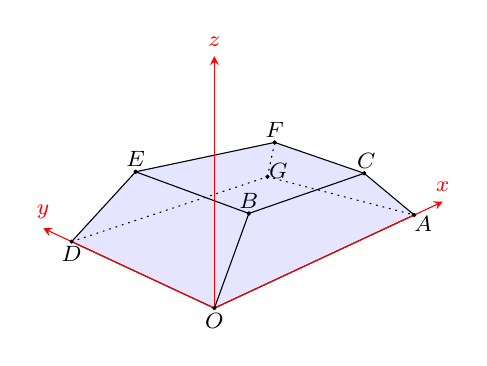
\begin{tikzpicture}[>=stealth, line join=round, line cap=round, 
			scale=.4, font=\footnotesize,
			declare function={r=3; a=75;}]
			% ve diem
			\path 
			(0,0) coordinate (O)
			(25:7) coordinate (A)
			(70:3.2) coordinate (B)
			(42:6.4) coordinate (C)
			(155:5) coordinate (D)
			(120:5) coordinate (E)
			(68:4.5) coordinate (G)
			(70:5.6) coordinate (F)
			;
			\fill[blue!10] (O)--(A)--(C)--(F)--(E)--(D)--(O);
			\draw (O)--(B)--(C)--(A) (O)--(D)--(E)--(B) (E)--(F)--(C) (D)--(O)--(A);
			\draw[dotted] (D)--(G)--(A) (G)--(F);
			\draw[->,red] (O)--(25:8) node[above]{$x$};
			\draw[->,red] (O)--(90:8) node[above]{$z$};
			\draw[->,red] (O)--(155:6) node[above]{$y$};
			\foreach \x/\g in {O/-90,B/90,C/80,A/-45,D/-90,E/90,G/30,F/90}{
				\draw[fill=black] (\x) circle (1.5pt)+(\g:.4) node{$\x$};}	
	\end{tikzpicture}
}
	\loigiai{
\begin{enumerate}
\item  Vì $B(4 k ; 3 k ; 2 k)$ thuộc mặt phẳng $(C B E F)\colon z=3$ nên $2 k=3 \Leftrightarrow k=\dfrac{3}{2}$.\\ Vậy $B\left(6 ; \dfrac{9}{2} ; 3\right)$.
\item Ta có $\vec{OA}=(50 ; 0 ; 0), \vec{OB}=\left(6 ; \dfrac{9}{2} ; 3\right)$ nên
$
\left[\vec{O A}, \vec{O B}\right]=(0 ;-150 ; 225)$.\\
Suy ra $\vec{n}=(0 ;-2 ; 3)$ là một véc-tơ pháp tuyến của mặt phẳng $(AOBC)$.\\
Vậy phương trình mặt phẳng $(AOBC)$ là
\[
0 \cdot(x-0)+(-2) \cdot(y-0)+3 \cdot(z-0)=0 \Leftrightarrow 2 y-3 z=0.\]
\item  Ta có $\vec{O D}=(0 ; 20 ; 0), \vec{OB}=\left(6 ; \dfrac{9}{2} ; 3\right)$ nên
\[
\left[\vec{OD}, \vec{OB}\right]=(60 ; 0 ;-120).\]
Suy ra $\vec{u}=(1 ; 0 ;-2)$ là một véc-tơ pháp tuyến của mặt phẳng $(DOBE)$.\\
Vậy phương trình mặt phẳng $(DOBE)$ là
\[
1 \cdot(x-0)+0 \cdot(y-0)+(-2) \cdot(z-0)=0 \Leftrightarrow x-2 z=0.\]
\item Một véc-tơ pháp tuyến của mỗi mặt phẳng $(A O B C)$ và $(D O B E)$ lần lượt là $\vec{p}=(0 ; 2 ;-3)$ và $\vec{q}=(-1 ; 0 ; 2)$.
\end{enumerate}
}
\end{vd}
\begin{vd}%[2H5V1-7]%[Dự án đề cương 3 khối NH24-25-Dot1-Huỳnh Đức Vũ]
	\immini
	{Hình vẽ bên minh họa một khu nhà đang xây dựng được gắn hệ trục tọa độ $Oxyz$ (đơn vị trên các trục là mét). Mỗi cột bê tông có dạng hình lăng trụ tứ giác đều và tâm của mặt đáy trên lần lượt là các điểm $A\left(2;1;3\right)$, $B\left(4;3;3\right)$, $C\left(6;3;2{,}5\right)$, $D\left(4;0;2{,}8\right)$.
		\begin{listEX}[1]
			\item Viết phương trình mặt phẳng $\left(ABC\right)$.
			\item Bốn điểm $A$, $B$, $C$, $D$ có đồng phẳng không?
	\end{listEX}}
	{%\includegraphics[scale=0.7]{images/Hinh21}
		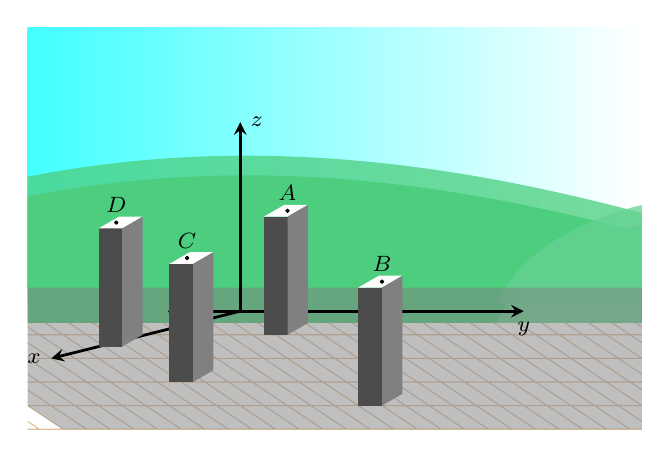
\begin{tikzpicture}[scale=0.3,font=\footnotesize, line join=round, line cap=round, >=stealth]
			%%%%%%%%%ICON
			\tikzset{Icon-mattroi/.pic={
					\def\r{0.35}
					\fill[opacity=1](0,0)circle(\r);
					\draw[line width=2*\r pt](0,0)circle(\r);
					\foreach \g in{1,...,10}{
						\draw[line width=\r pt](\g*36:1.2*\r)++(\g*36:0.1*\r)--++(\g*36:\r*0.25);
					}
			}}
			%%%%%%%%%%%%%%%%%%%MÁy bay
			\tikzset{Icon-Maybay/.pic={
					\begin{scope}
						\fill[ball color =cyan!40!gray,rounded corners=0.02](-5.6,3)--++(60:0.8)--++(2:0.55)--++(-90:2)--cycle;
						%%Hai cánh
						\fill[ball color =cyan!90!gray!40!white](-0.4,1.5)..controls++(75:2)and++(-68:0.75)..(-0.15,4)--++(-5:0.35)..controls++(-50:0.95)and++(106:2)..(1.25,1.5)--cycle;
						%Thân
						\fill[ball color =cyan!30!gray](-4.85,1)..controls++(-90:0.6) and++(180:0.2)..(-4,0.5)--++(-12:3.3)--++(0:4)..controls++(0:2) and++(-172:1)..(6,0)..controls++(8:1)and++(-90:0.1)..(6.85,0.3)..controls++(90:0.2) and++(-30:1)..(5,1.3)..controls++(90:0.25) and++(0:8)..(-4,1.5)--cycle;
						\draw[cyan!40!black](6.85,0.3)coordinate(mui)..controls++(-90:0.5) and++(0:6)..(-2,0.2);
						% Cánh phải
						\fill[ball color =cyan!90!gray!40!white,rounded corners=0.02](-1.8,0)--++(-5:0.35)--++(-147:4.85)--++(-50:0.7)--++(25.5:6.5)..controls++(-155.5:0.5) and++(-170:0.15)..(1.5,-0.25)..controls++(120:0.5) and++(2:1)..(-1.8,0);
						\fill[ball color =cyan!90!gray!40!white,rounded corners=0.02](-6.1,-2.3)--++(-54:0.7)--++(-28:0.7)--++(25.5:.35)--++(-180:.2)--++(135:1.2)--cycle;
						%%Thân đuôi
						\fill[ball color =cyan!90!gray!40!white,rounded corners=0.02](-6.9,3.6)--++(2:1)..controls++(-35:2) and++(178:2.3)..(-2,1.5)..controls++(-90:0.2) and++(20:1)..(-3.5,1)--++(180:1.2)--cycle;
						%%Đuôi
						\fill[ball color =cyan!90!gray!40!white,rounded corners=0.02](-6,2.5)--++(0:1.35)--++(-156:2.5)--++(170:0.75)--cycle;
						\fill[ball color =cyan!70!gray!40!white,rounded corners=0.02](-1.9,-0.17)--++(90:0.72)--++(181:2.45)--++(-90:0.6)--cycle;
						\fill[ball color =cyan!90!gray!10!black,line width=0.02,draw=cyan!30!black,rounded corners=0.005](-1.9,-0.18)arc(-90:270:0.2 and 0.38);
						%%Cửa kính
						\fill[cyan](5.05,1.3)--++(-25:0.8)..controls++(-140:0.55)and++(10:0.5)..(4.2,0.6)..controls++(180:0.15) and++(182:0.45)..(4.3,1.1)..controls++(2:0.5) and++(-135:0.2)..(5.1,1.3);
						\draw[draw=teal,double,distance=0.03](5.05,1.3)++(-26:0.8)..controls++(-140:0.55)and++(10:0.5)..(4.2,0.6)foreach \i in{1,2,...,4}{coordinate[pos=\i/4](B\i)}..controls++(180:0.15) and++(182:0.45)..(4.3,1.1)..controls++(2:0.5) and++(-135:0.2)..(5.1,1.3)foreach \i in{1,2,...,10}{coordinate[pos=\i/10](A\i)}(A2)--(B2)(A6)--(B1);
						%Ô cửa trên thân máy bay
						\foreach \i in {0,1,...,6}
						\fill[ball color=cyan](-0.8+0.5*\i,0.4)arc(-90:270:0.1 and 0.2);
						\fill[draw=cyan!10!teal,ball color=cyan!80!gray,rounded corners=0.015](3.2,-0.2)--++(95:0.9)--++(0:0.5)--++(-85:0.9)--cycle;\end{scope}
			}}
			
			%%%%%%%%%%%%%
			\tikzset{Icon-may/.pic={
					\def\r{0.35}
					\fill[white,line width=2.5*\r pt](-\r,0)--(\r,0)..controls++(0:\r) and ++(30:\r)..(0.8*\r,\r)..controls++(100:\r) and ++(80:\r)..(-0.75*\r,0.8*\r)..controls++(140:\r) and++(180:\r)..(-\r,0);
			}}
			
			%\path(0,0)node[opacity=1]{\includegraphics[scale=0.25]{Hoa-Atiso.png}};
			\clip(-11,-7)rectangle(15,10);
			\fill[left color=cyan](-20,-1)rectangle(15,10);
			\draw[brown,xslant=-1.5,opacity=0.5](-25,-8)grid(15,-1);
			%\draw[red](-5,-5)grid(5,5);
			\tikzset{Back/.pic={
					\foreach \x/\y in{1/-0.5,0.75/0}{
						\begin{scope}[shift={(0.25,\y)},opacity=\x,xscale=1.35]
							\fill[green!45!teal!70!white,shift={(-10,0)}](2,-1)..controls++(80:3) and++(130:2)..(6,1)..controls++(45:5) and++(140:3)..(15,0)..controls++(70:1) and++(105:1)..(18,-1)--cycle;
							\fill[green!40!teal!60!white](2,-1)..controls++(80:3) and++(130:2)..(6,1)..controls++(45:5) and++(140:3)..(15,0)..controls++(70:1) and++(105:1)..(18,-1)--cycle;
						\end{scope}
			}}}
			\tikzset{cot/.pic={
					\path(0,0)coordinate(A)(1,0)coordinate(B)++(30:1)coordinate(C)(A)++(30:1)coordinate(D);
					\path[shift={(0,5)}](0,0)coordinate(A')(1,0)coordinate(B')++(30:1)coordinate(C')(A')++(30:1)coordinate(D');
					\fill[gray!60!black](A)--(B)--(B')--(A')--cycle;
					\fill[gray!0.5](A')--(B')--(C')--(D')--cycle;
					\fill[gray](B)--(B')--(C')--(C)--cycle;
			}}
			\path(-1,0)pic[yscale=0.5]{Back};
			\fill[gray,xslant=-1.5,opacity=0.5](-20,-7)rectangle(15,-1);
			%\path(5,6)pic{Icon-may}(8,5.5)pic[scale=1]{Icon-may}(-6,6)pic[scale=1]{Icon-may}(8.5,7.5)pic[yellow,scale=1.5]{Icon-mattroi}(-9,2)pic[scale=0.5]{Icon-cotden}(6,2)pic[scale=0.5]{Icon-cotden}(14,2)pic[scale=0.5]{Icon-cotden}(-2,7)pic[scale=0.15]{Icon-Maybay};
			\begin{scope}[line width=1pt]
				\draw[-stealth](-5,-2)--(10,-2)node[below]{$y$};
				\draw[-stealth](-2,-2)--(-10,-4)node[left]{$x$};
				\draw[-stealth](-2,-2)--(-2,6)node[right]{$z$};
			\end{scope}
			%%%%%%%%%%%%%%%%%%%%
			\path(-1,-3)pic[scale=0.3]{cot}(3,-6)pic[scale=0.3]{cot}(-5,-5)pic[scale=0.3]{cot}(-8,-3.5)pic[scale=0.3]{cot};
			\draw[fill]([shift={(1,5.25)}]-1,-3)circle(2pt)node[scale=1,above]{$A$}
			([shift={(1,5.25)}]3,-6)circle(2pt)node[scale=1,above]{$B$}
			([shift={(0.75,4.25)}]-5,-4.0)circle(2pt)node[scale=1,above]{$C$}(-2.75,-2.5)([shift={(0.75,4.25)}]-8,-2.5)circle(2pt)node[scale=1,above]{$D$};
	\end{tikzpicture}}
	\loigiai{
		\begin{enumerate}
			\item Ta có $\vec{AB}=\left(2;2;0\right)$, $\vec{AC}=\left(4;2;-\dfrac{1}{2}\right)$ suy ra $\vec{n}=\left[\vec{AB},\vec{AC}\right]=\left(-1;1;-4\right)$.\\
			Mặt phẳng $\left(ABC\right)$ đi qua $A\left(2;1;3\right)$ và nhận $\vec{n}=\left(-1;1;-4\right)$ làm véc-tơ pháp tuyến nên có phương trình
			$$-1\cdot \left(x-2\right)+1\cdot \left(y-1\right)-4\cdot \left(z-3\right)=0 \Leftrightarrow -x+y-4z+13=0.$$ 
			\item Thay tọa độ $D\left(4;0;2{,}8\right)$  vào phương trình mặt phẳng $\left(ABC\right)$ ta thấy không thỏa mãn nên điểm $D$ không thuộc mặt phẳng $\left(ABC\right)$.
		\end{enumerate}
	}
\end{vd}
\begin{vd}%[2H5V1-7]%[Dự án đề cương 3 khối NH24-25-Dot1-Huỳnh Đức Vũ]
	\immini{Hình vẽ bên minh hoạ hình ảnh hai mái nhà của một nhà kho trong không gian với hệ toạ độ $Oxyz$ (đơn vị trên mỗi trục toạ độ là mét). Các bức tường của nhà kho đều được xây vuông góc với mặt đất.
		\begin{enumerate}[a)]
			\item Lập phương trình của hai mặt phẳng tương ứng mỗi mái nhà.
			\item Tìm tọa độ của điểm $Q$.
			\item Tìm toạ độ của véc-tơ $\vec{PQ}$.
	\end{enumerate} }{
		\begin{tikzpicture}[line join = round, line cap = round,>=stealth,font=\footnotesize,scale=.3,declare function={gx=30;gy=140;gop=atan(6/5);op=sqrt(5^2+6^2);}]
			\path 
			(0,0) coordinate (O)
			(0,9) coordinate (D)
			(gx:5) coordinate (P1)
			($(P1)+(0,6)$) coordinate (P)
			(gx:11) coordinate (A1)
			($(A1)+(0,9)$) coordinate (A)
			(gy:14) coordinate (C1)
			($(C1)+(0,9)$) coordinate (C)
			($(C)-(D)+(P)$) coordinate (Q)
			($(Q)-(P)+(A)$) coordinate (B)
			($(B)-(0,9)$) coordinate (B1)
			(gx:13) coordinate (x)
			(gy:17) coordinate (y)
			(0,20) coordinate (z)
			;
			\draw[->,>=stealth] (O)node[below]{$O$}--(x)node[below]{$x$};
			\draw[->,>=stealth] (O)--(y)node[left]{$y$};
			\draw[->,>=stealth] (O)--(z)node[right]{$z$};
			\draw (C1)--(C)node[above]{$C(0;20;10)$}--(Q)--(B)node[above]{$B(10;20;10)$}--(A)--(P)--(D)node[below left]{$D(0;0;9)$}--(C) (A)node[right]{$A(10;0;9)$}--(A1) (Q)--(P)node[shift={(-0.2,-0.4)}]{$P\left(5;0;6\right)$};
			\draw[dashed] (C1)--(B1)--(A1) (B)--(B1);
			\foreach \x/\gm in {D/180,P/90,A/0,C/90,Q/0,B/90,O/-90} \fill (\x) circle (3pt);
	\end{tikzpicture}}
	\loigiai{
		\begin{enumerate}[a)]
			\item Hai mặt phẳng tương ứng mỗi mái nhà là $\left(ABP\right)$ và $\left(CDP\right)$.
			\begin{itemize}
				\item Do mặt phẳng $\left(ABP\right)$ có cặp véc-tơ chỉ phương là $\vec{AB}=\left(0;20;1\right)$, $\vec{AP}=\left(-5;0;-3\right)$ nên có một véc-tơ pháp tuyến là
				\[\left[\vv{AB},\vv{AP}\right]=\left(\begin{vmatrix}
					20 & 1\\
					0 & -3
				\end{vmatrix};
				\begin{vmatrix}
					1 & 0\\
					-3 & -5
				\end{vmatrix};
				\begin{vmatrix}
					0 & 20\\
					-5 & 0
				\end{vmatrix}
				\right)=\left(-60;-5;100\right).\]	
				Mà mặt phẳng $\left(ABP\right)$ đi qua điểm $A\left(10;0;9\right)$ nên có phương trình là
				$$-60\cdot\left(x-10\right)-5\cdot\left(y-0\right)+100\cdot\left(z-9\right)=0 \Leftrightarrow 12x+y-20z+60=0.$$
				\item Do mặt phẳng $\left(CDP\right)$ có cặp véc-tơ chỉ phương là $\vec{DP}=\left(5;0;-3\right)$, $\vec{DC}=\left(0;20;1\right)$ nên có một véc-tơ pháp tuyến là
				$$\left[\vec{DP},\vec{DC}\right]=\left(\left|\begin{array}{cc}
					0 & -3\\
					20 & 1
				\end{array}\right|;\left|\begin{array}{cc}
					-3 & 5\\
					1 & 0
				\end{array}\right|;\left|\begin{array}{cc}
					5 & 0\\
					0 & 20
				\end{array}\right|\right)=(60;-5;100).$$
				Mà mặt phẳng $(CDP)$ đi qua điểm $D(0;0;9)$ nên có phương trình là
				$$60(x-0)-5(y-0)+100(z-9)=0 \Leftrightarrow 12x-y+20z-180=0.$$
			\end{itemize}
			\item Vì các bức tường của nhà kho đều được xây vuông góc với mặt đất nên với hệ tọa độ trên ta có $Q(x;20;z)$.\\
			Do điểm $Q$ thuộc mặt phẳng $(ABP)$ nên tọa độ của điểm $Q$ thoả mãn $12x+20-20z+60=0$ tức là $3x-5z=-20$.\\
			Do điểm $Q$ thuộc mặt phẳng $(CDP)$ nên tọa độ của điểm $Q$ thoả mãn $12x-20+20z-180=0$, tức là $3x+5z=50$.\\
			Ta có hệ phương trình $\heva{&3x-5z=-20\\&3x+5z=50} \Leftrightarrow \heva{&x=5\\&z=7.}$\\
			Vậy $Q(5;20;7)$.
			\item Với $P(5;0;6)$ và $Q(5;20;7)$ ta có $\vec{PQ}=(0;20;1)$.
		\end{enumerate}
	}
\end{vd}
\subsection{BÀI TẬP RÈN LUYỆN}
\subsubsection{BÀI TẬP TRẮC NGHIỆM NHIỀU LỰA CHỌN}
\Opensolutionfile{ans}[ans/ansABCD]
\begin{ex}%[2H5H1-2]%[Dự án đề cương 3 khối NH24-25-Dot1-Huỳnh Đức Vũ]
	Trong không gian $Oxyz$, cho ba điểm $A(2;1;-1)$, $B(3;0;1)$, $C(2;-1;3)$. Một véc-tơ pháp tuyến của mặt phẳng $(ABC)$ là
	\choice
	{\True $\vec{n}_1=(0;-4;-2)$}
	{$\vec{n}_2=(0;4;-2)$}
	{$\vec{n}_3=(1;-1;2)$}
	{$\vec{n}_4=(0;-2;4)$}
	\loigiai{
		Mặt phẳng $(ABC)$ có cặp véc-tơ chỉ phương là $\vec{AB}=(1;-1;2)$, $\vec{AC}=(0;-2;4)$ nên có một véc-tơ pháp tuyến là $$\vec{n}=\left[\vec{AB},\vec{AC}\right]=(0;-4;-2).$$
	}
\end{ex}
\begin{ex}[Trích Đề cuối kì 2 – THPT Phạm Văn Đồng – Quảng Ngãi - Năm học 2024 – 2025]%[2H5N1-5]%[Dự án đề cương 3 khối NH24-25-Dot1-Huỳnh Đức Vũ]
	Trong không gian $Oxyz$, khoảng cách từ điểm $M(9;7;8)$ đến mặt phẳng $(P)\colon ax + by + cz + d = 0$ bằng
	\choice
	{$\dfrac{\left|7a + 8b + 9c + d\right|}{\sqrt{7^2 + 8^2 + 9^2}}$}
	{$\dfrac{\left|9a + 7b + 8c + d\right|}{\sqrt{9^2 + 7^2 + 8^2}}$}
	{$\dfrac{\left|7a + 8 b + 9c + d\right|}{\sqrt{a^2 + b^2 + c^2}}$}
	{\True $\dfrac{\left|9a + 7b + 8c + d\right|}{\sqrt{a^2 + b^2 + c^2}}$}
	\loigiai{
		Khoảng cách từ điểm $M$ đến mặt phẳng $(P)$ được tính theo công thức:
		\[\mathrm{d}\left(M,(P)\right)=\dfrac{\left|a x_0+b y_0 + cz_0 + d\right|}{\sqrt{a^2 + b^2 + c^2}}.\]
		Thay tọa độ điểm $M(9;7;8)$ vào công thức trên ta được $\mathrm{d}\left(M,(P)\right)=\dfrac{\left|9a + 7b + 8c + d\right|}{\sqrt{a^2 + b^2 + c^2}}$.
	}
\end{ex}
\begin{ex}[Trích Đề cuối kì 2 – THPT Nguyễn Hữu Cầu – HCM – Năm học 2024 – 2025]%[2H5N1-1]%[Dự án đề cương 3 khối NH24-25-Dot1-Huỳnh Đức Vũ]
	Trong không gian với hệ trục $Oxyz$, cho mặt phẳng $(P)\colon 2x + y - z + 3 = 0$. Điểm nào sau đây không thuộc mặt phẳng $(P)$?
	\choice
	{$M(-2; 0; 1)$}
	{\True $N(0; -1; 2)$}
	{$P(-1; 0; 1)$}
	{$Q(1; -4; 1)$}
	\loigiai{
	Thay lần lượt tọa độ các điểm $M$, $N$, $P$, $Q$ vào phương trình của mặt phẳng $(P)$, ta thấy chỉ có điểm $N(-2;0;1)$ không thỏa mãn nên điểm $N(-;0;1)$ không thuộc mặt phẳng $(P)$.
	}
\end{ex}
\begin{ex}%[2H5N1-4]%[Dự án đề cương 3 khối NH24-25-Dot1-Huỳnh Đức Vũ]
	Trong không gian $Oxyz$, mặt phẳng $(\alpha)\colon x+2y+3z-6=0$ cắt trục $Oy$ tại điểm có tung độ bằng
	\choice
	{$2$}
	{\True $3$}
	{$6$}
	{$1$}
	\loigiai
	{
		Mặt phẳng $(\alpha)\colon x+2y+3z-6=0$ cắt trục $Oy$ tại điểm $A(0;y_0;0)$.\\
		Khi đó $0+2y_0+3\cdot 0-6=0\Leftrightarrow y_0=3$.
	}
\end{ex}
\begin{ex}%[2H5H1-7]%[Dự án đề cương 3 khối NH24-25-Dot1-Huỳnh Đức Vũ]
	Trong không gian $Oxyz$, cho mặt phẳng $\left(P\right)$ có phương trình $\dfrac{x}{-2}+\dfrac{y}{-1}+\dfrac{z}{3}=1$ cắt ba trục $Ox$, $Oy$, $Oz$ lần lượt tại $A$, $B$, $C$. Khi đó thể tích của khối chóp $OABC$ bằng
	\choice
	{$3$}
	{\True $1$}
	{$6$}
	{$2$}
	\loigiai{
		Ta có $A=Ox\cap \left(P\right)\Rightarrow A\left(-2; 0; 0\right)\Rightarrow OA=2$.\\
		$B=Oy\cap \left(P\right)\Rightarrow B\left(0;-1; 0\right)\Rightarrow OB=1$.\\
		$C=Oz\cap \left(P\right)\Rightarrow C\left(0; 0; 3\right)\Rightarrow OC=3$.\\
		Vì $OA$, $OB$, $OC$ đôi một vuông góc nên $V_{OABC}=\dfrac{1}{6} OA\cdot OB\cdot OC=1$.
	}

\end{ex}
\begin{ex}[Trích Đề Giữa kì 2 – THPT- thị xã Quảng Trị - Năm học 2024-2025]%[2H5H1-3]%[Dự án đề cương 3 khối NH24-25-Dot1-Huỳnh Đức Vũ]
	Trong không gian $Oxyz$, cho hai điểm $A(1; 3; -4)$ và $B(-1; 2; 2)$. Viết phương trình mặt phẳng trung trực $(\alpha)$ của đoạn thẳng $AB$.
	\choice
	{$(\alpha) \colon 4x + 2y + 12z + 7 = 0$}
	{$(\alpha) \colon 4x - 2y - 12z - 7 = 0$}
	{\True $(\alpha) \colon 4x + 2y - 12z - 17 = 0$}
	{$(\alpha) \colon 4x - 2y + 12z + 17 = 0$}
	\loigiai{
		Mặt phẳng $(\alpha)$ nhận $\vec{AB}=(-2;-1;6)$ là một véc-tơ pháp tuyến của mặt phẳng và đi qua trung điểm $I\left(0;\dfrac{5}{2};-1\right)$ của đoạn thẳng $AB$. Phương trình mặt phẳng $(\alpha)$ là
		\[-2(x-0)-1\left(y-\dfrac{5}{2}\right)+6(z+1)=0 \Leftrightarrow -2x-y+6z+\dfrac{17}{2}=0 \Leftrightarrow 4x + 2y -12z - 17 = 0.\]}

\end{ex}

\begin{ex}[Lớp 12 - Đề giữa học kì 2 - THPT Chuyên Lê Quý Đôn - Ninh Thuận]%[2H5H1-2]%[Dự án đề cương 3 khối NH24-25-Dot1-Huỳnh Đức Vũ]
	Trong không gian với hệ trục $Oxyz$, cho ba điểm $A(2;-1;3)$, $B(4;0;1)$, $C(-10;5;3)$. Một véc-tơ pháp tuyến của mặt phẳng $(ABC)$ là
	\choice
	{$\vec{n}=(1;2;0)$}
	{$\vec{n}=(1;8;2)$}
	{$\vec{n}=(1;-2;2)$}
	{\True $\vec{n}=(1;2;2)$}
	\loigiai{
		Ta có $\vec{AB}=(2;1;-2)$ và $\vec{AC}=(-12;6;0)$.\\
		Suy ra $\left[\vec{AB},\vec{AC}\right]=(12;24;24)=12\vec{n}$, với $\vec{n}=(1;2;2)$.\\
	Vậy véc-tơ $\vec{n}=(1;2;2)$ là một véc-tơ pháp tuyến của mặt phẳng $(ABC)$.	
	}
\end{ex}

\begin{ex}[Trích Đề Giữa kì 2 – THPT Việt Nam Ba Lan - Tp Hà Nội-Năm học 2024-2025]%[2H5H1-3]%[Dự án đề cương 3 khối NH24-25-Dot1-Huỳnh Đức Vũ]
	Trong không gian $Oxyz$, phương trình của mặt phẳng đi qua điểm $B(2;1;-3)$ đồng thời vuông góc với hai mặt phẳng $(P) \colon x+y+3z=0$ và $(Q) \colon 2x-y+z=0$ là
	\choice
	{\True $4x + 5y - 3z - 22 = 0$}
	{$4x - 5y - 3z - 12 = 0$}
	{$4x + 5y + 3z - 4 = 0$}
	{$4x - 5y + 3z + 6 = 0$}
	\loigiai{
		Gọi $(\alpha)$ là mặt phẳng cần tìm. Vì $(\alpha)$ vuông góc với $(P)$ và $(Q)$ nên một véc-tơ pháp tuyến của mặt phẳng $(\alpha)$ là
		$$\vec{n}=\left[\vec{n}_P, \vec{n}_Q\right]=(4;5;-3).$$
	Mặt phẳng $(\alpha)$ đi qua điểm $B(2;1;-3)$ và nhận véc-tơ 
	$\vec{n}=(4;5;-3)$ làm véc-tơ pháp tuyến nên có phương trình là
	$$4(x-2)+5(y-1)-3(z+3)=0 \Leftrightarrow 4x+5y-3z-22=0.$$
	}
	%<MyLT1>
\end{ex}

\begin{ex}[Trích Đề cuối kì 2 – THPT Phan Bội Châu-Bình Thuận -Năm học 2024-2025]%[2H5H1-4]%[Dự án đề cương 3 khối NH24-25-Dot1-Huỳnh Đức Vũ]
	Trong không gian $Oxyz$, cho hai mặt phẳng $(P)\colon 2x+y-3z-2024=0$ và $(Q)\colon x+m y+z+2025=0$ với $m$ là tham số. Mặt phẳng $(P)$ vuông góc với mặt phẳng $(Q)$ khi và chỉ khi
	\choice
	{$m=5$}
	{\True $m=1$}
	{$m=-1$}
	{$m=-5$}
	\loigiai{
		Mặt phẳng $(P)$ có một véc-tơ pháp tuyến là $\vec{n}_1=(2;1;-3)$.\\
		Mặt phẳng $(Q)$ có một véc-tơ pháp tuyến là $\vec{n}_2=(1;m;1)$.\\
		Khi đó \allowdisplaybreaks
		\begin{eqnarray*}
			& & (P)\perp (Q)\\
			&\Leftrightarrow & \vec{n}_1\cdot\vec{n}_2=0\\
			&\Leftrightarrow & 2\cdot 1+ 1\cdot m + (-3)\cdot 1=0\\
			&\Leftrightarrow & m=1.
		\end{eqnarray*}
	}
	
\end{ex}

\begin{ex}%[2H5H1-3]%[Dự án đề cương 3 khối NH24-25-Dot1-Huỳnh Đức Vũ]
	Trong không gian $Oxyz$, mặt phẳng đi qua điểm $M(1;-2; 3)$ và song song với mặt phẳng $(Q) \colon 2x-3y+z+5=0$ có phương trình là
	\choice
	{\True $2x-3y+z-11=0$}
	{$2x-3y+z+11=0$}
	{$x-2y+3z-11=0$}
	{$x-2y+3z+11=0$}
	\loigiai{
		Mặt phẳng song song với mặt phẳng $(Q)$ có dạng $2x-3y+z+d=0$ $(d \neq 5)$.\\
		Mặt phẳng này đi qua điểm $M(1;-2;3)$ nên $2\cdot 1-3 \cdot (-2)+3+d=0 \Rightarrow d=-11$.\\
		Vậy mặt phẳng cần tìm có phương trình là $2x-3y+z-11=0$.
	}
\end{ex}

\begin{ex}%[2H5H1-4] %[2H5H1-3]%[Dự án đề cương 3 khối NH24-25-Dot1-Huỳnh Đức Vũ]
	Trong không gian $Oxyz$ cho hai mặt phẳng $(\alpha)\colon (m+1)x+(m-1)y+6z-4=0$ và $(\beta)\colon 2x+y+3z-3=0$. Giá trị của $m$ để hai mặt phẳng $(\alpha)$ và $(\beta)$ song song với nhau bằng
	\choice
	{\True $m=3$}
	{$m=1$}
	{$m=2$}
	{$m=-1$}
	\loigiai
	{Ta có véc-tơ pháp tuyến của $(\alpha)$ là $\vec{n}_1=(m+1;m-1;6)$, véc-tơ pháp tuyến của $(\beta)$ là $\vec{n}_2=(2;1;3)$.\\
	Hai mặt phẳng $(\alpha)$ và $(\beta)$ song song khi và chỉ khi 
	\[\dfrac {m+1}{2}=\dfrac {m-1}{1}=\dfrac {6}{3}\ne \dfrac {-4}{-3}\Rightarrow m=3.\]}	
\end{ex}
\begin{ex}[Trích Đề cuối kì 2 – THPT Ngô Quyền-TP.HCM-Năm học-2024-2025]%[2H5H1-5]%[2H5H1-3]%[Dự án đề cương 3 khối NH24-25-Dot1-Huỳnh Đức Vũ]
	Trong không gian $Oxyz$, khoảng cách từ điểm $A(1;0;0)$ tới mặt phẳng $(P)\colon 2x+2y-z+1=0$ bằng
	\choice
	{\True $1$}
	{$9$}
	{$\sqrt{3}$}
	{$3$}
	\loigiai{
		Khoảng cách từ điểm $A(1;0;0)$ tới mặt phẳng $(P)\colon 2x+2y-z+1=0$ là $$\mathrm{d}(A,(P))=\dfrac{\left|2\cdot1+2\cdot0-0+1\right|}{\sqrt{2^2+2^2+(-1)^2}}=\dfrac{\left|3\right|}{\sqrt{9}}=1.$$}
\end{ex}
\begin{ex}[Trích Đề cuối kì 2 – THPT Trí Đức - TPHCM – Năm học 2024-2025]%[2H5H1-6]%[Dự án đề cương 3 khối NH24-25-Dot1-Huỳnh Đức Vũ]
	Trong không gian $Oxyz$, khoảng cách giữa hai mặt phẳng $(P)\colon x+2y+2z-10=0$ và $(Q)\colon x+2y+2z-5=0$ bằng
	\choice
	{\True $\dfrac{5}{3}$}
	{$5$}
	{$\dfrac{7}{3}$}
	{$\dfrac{5}{9}$}
	\loigiai{
		Ta thấy hai mặt phẳng $(P)\colon x+2y+2z-10=0$ và $(Q)\colon x+2y+2z-5=0$ đều có véc-tơ pháp tuyến $(1;2;2)$ và $-10\neq-5$ nên hai mặt phẳng $(P)\colon x+2y+2z-10=0$ và $(Q)\colon x+2y+2z-5=0$ song song với nhau.\\
		Lấy điểm $A(2;2;2)\in (P)$.\\
		Khi đó, khoảng cách giữa hai mặt phẳng $(P)$ và $(Q)$ là
		\begin{eqnarray*}
			\mathrm{d}((P),(Q))=\mathrm{d}(A,(Q))=\dfrac{\left|2+2\cdot2+2\cdot2-5 \right|}{\sqrt{1^2+2^2+2^2}}=\dfrac{5}{3}.
		\end{eqnarray*}
		}
\end{ex}
\begin{ex}%[2H5H1-3]%[Dự án đề cương 3 khối NH24-25-Dot1-Huỳnh Đức Vũ]
		Trong không gian $Oxyz$, cho các mặt phẳng $(Q)\colon x+y+3 z=0$, $(R)\colon 2x-y+z=0$ và điểm $B(2;1;-3)$. Mặt phẳng $(P)$ đi qua điểm $B$ đồng thời vuông góc với hai mặt phẳng $(Q)$ và $(R)$ có phương trình là
	\choice
	{$4x+5y-3z+22=0$}
	{$4x-5y-3z-12=0$}
	{$2x+y-3z-14=0$}
	{\True $4x+5 y-3z-22=0$}
	\loigiai{
		Hai mặt phẳng $(Q)$ và $(R)$ có véc-tơ pháp tuyến lần lượt là $\vec{n}_Q=(1;1;3)$ và $\vec{n}_R=(2;-1;1)$.\\
		Mặt phẳng $(P)$ đồng thời vuông góc với hai mặt phẳng $(Q)$ và $(R)$ nên có một véc-tơ pháp tuyến là $\vec{n}_P=(4;5;-3)$.\\
		Mặt phẳng $(P)$ có phương trình là
		$$4\cdot(x-2)+5\cdot(y-1)-3(z+3)=0 \text { hay } 4x+5y-3z-22=0.$$
	}
\end{ex}
\begin{ex}[Trích Đề cuối kì 2 – THPT Nguyễn Hữu Cầu-TP.HCM -Năm học-2024-2025]%[2H5H1-3]%[Dự án đề cương 3 khối NH24-25-Dot1-Huỳnh Đức Vũ]
Trong không gian $Oxyz$, mặt phẳng $(P)$ đi qua điểm $A(-1;-2;2)$ và chứa trục $Oz$, có một véc-tơ pháp tuyến $\vec{n}= (1; a; b)$. Giá trị của $a + b$ là
\choice
{$-2$}
{\True $-\dfrac{1}{2}$}
{$-\dfrac{3}{2}$}
{$-1$}
\loigiai{
Mặt phẳng $(P)$ chứa trục $Oz$ véc-tơ pháp tuyến của $(P)$ vuông góc với véc-tơ đơn vị của trục $Oz$. Do đó, ta có 
\[\vec{n} \cdot \vec{u} = 0 \Rightarrow 1 \cdot 0 + a \cdot 0 + b \cdot 1 = 0 \Rightarrow b = 0.\]
Suy ra $\vec{n} = (1; a; 0)$.\\
Vì mặt phẳng $(P)$ đi qua điểm $A(-1; -2; 2)$ và có pháp tuyến $\vec{n} = (1; a; 0)$ nên phương trình mặt phẳng là
	$$1\cdot(x + 1) + a\cdot(y + 2) + 0\cdot(z - 2) = 0 \Rightarrow x + 1 + a\cdot(y + 2) = 0.$$
Mặt phẳng $(P)$ chứa trục $Oz$ nên $(P)$ chứa điểm $O(0; 0; 0)$. Thay tọa độ điểm $O$ vào phương trình của $(P)$, ta được
	$$0 + 1 + a\cdot(0 + 2) = 0 \Rightarrow 1 + 2a = 0 \Rightarrow a = -\dfrac{1}{2}.$$
	Vì $b = 0$ nên $a + b = -\dfrac{1}{2} + 0 = -\dfrac{1}{2}$.
}
\end{ex}
%\begin{ex}%[2H5N1-5]%[Dự án đề cương 3 khối NH24-25-Dot1-Huỳnh Đức Vũ]
%	Trong không gian với hệ tọa độ $Oxyz$, cho điểm $A(1;-1;1)$ và mặt phẳng $(P)\colon -x+2y-2z+11=0$. Gọi $(Q)$ là mặt phẳng song song $(P)$ và cách $A$ một khoảng bằng $2$. Tìm phương trình mặt phẳng $(Q)$.
%	\choice
%	{$(Q)\colon x-2y+2z+1=0$}
%	{\True$(Q)\colon x-2y+2z+1=0$ và $(Q)\colon -x+2y-2z-11=0$}
%	{$(Q)\colon -x+2y-2z+11=0$}
%	{$(Q)\colon x-2y+2z-11=0$}
%	\loigiai{
%		Do $(Q)$ là mặt phẳng song song $(P)$ nên ptmp $(Q)\colon -x+2y-2z+D=0$.\\
%		Ta có $\mathrm{d}\left(A,(Q)\right)=2\Leftrightarrow\dfrac{|-1-2-2+D|}{3}=2 \Leftrightarrow|D-5|=6\Leftrightarrow\hoac{&D=11\\&D=-1.} $ \\
%		Vậy có hai mặt phẳng $(Q)$ thỏa mãn yêu cầu đề bài.}
%\end{ex}
\begin{ex}%[2H5N1-5]%[Dự án đề cương 3 khối NH24-25-Dot1-Huỳnh Đức Vũ]
	Trong không gian $Oxyz$, hai mặt phẳng $4x-4y+2z-7=0$ và $2x-2y+z+4=0$ chứa hai mặt của hình lập phương. Thể tích khối lập phương đó bằng
	\choice
	{$V=\dfrac{81\sqrt{3}}{8}$}
	{\True $V=\dfrac{125}{8}$}
	{$V=\dfrac{9\sqrt{3}}{2}$}
	{$V=\dfrac{27}{8}$}
	\loigiai
	{Ta có $\dfrac{4}{2}=\dfrac{-4}{-2}=\dfrac{2}{1}\neq \dfrac{-7}{4}$ nên hai mặt phẳng $(P)\colon4x-4y+2z-7=0$ và $(Q)\colon2x-2y+z+4=0$ song song với nhau.\\
		Suy ra khoảng cách giữa hai mặt phẳng bằng độ dài cạnh của hình lập phương.\\
		Chọn $M(0;0;-4)\in(Q)$ suy ra
		\[\mathrm{d}((P),(Q))=\mathrm{d}(M,(P))=\dfrac{|4\cdot0-4\cdot0+2\cdot(-4)-7|}{\sqrt{4^2+(-4)^2+2^2}}=\dfrac{5}{2}.\]
		Vậy thể tích khối lập phương đã cho là $V=\left(\dfrac{5}{2}\right)^3=\dfrac{125}{8}$.
	}
\end{ex}
\begin{ex}%[2H5N1-5]%[Dự án đề cương 3 khối NH24-25-Dot1-Huỳnh Đức Vũ]
	Trong không gian với hệ trục tọa độ $Oxyz$, cho 2 mặt phẳng $(P) \colon x + y - z + 1 = 0$ và $(Q) \colon x - y + z - 5 = 0$. Có bao nhiêu điểm trên trục $Oy$ thỏa mãn điểm $M$ cách đều 2 mặt phẳng $(P)$ và $(Q)$.
	\choice
	{\True $1$}
	{$2$}
	{$3$}
	{$0$}
	\loigiai{
		Điểm $M \in Oy \Rightarrow M(0; m; 0)$. \\
		$\mathrm{d}(M,(P))=\mathrm{d}(M,(Q)) \Leftrightarrow \dfrac{\left|m + 1\right|}{\sqrt{3}} = \dfrac{\left|m + 5\right|}{\sqrt{3}} \Leftrightarrow m = -3$.\\ Vậy có $1$ điểm $M$  thỏa mãn yêu cầu của bài toán.
	}
\end{ex}
\begin{ex}%[2H5N1-5]%[Dự án đề cương 3 khối NH24-25-Dot1-Huỳnh Đức Vũ]
	Trong không gian $Oxyz$, cho ba điểm $A(1;0;0)$, $B(0;2;0)$ và $C(0{,}0,3)$. Khoảng cách từ gốc tọa độ đến mặt phẳng $(ABC)$ bằng
	\choice
	{\True $\dfrac{6}{7}$}
	{$\dfrac{6}{11}$}
	{$\dfrac{3}{5}$}
	{$\dfrac{1}{3}$}
	\loigiai{
		\textbf{Cách 1}. Ta có $\vec{AB}=(-1;2;0),\vec{AC}=(-1;0;3)$ $\Rightarrow\vec{n}=\left[\vec{AB,}\vec{AC}\right]=(6;3;2)$ là một véc-tơ pháp tuyến của mặt phẳng $(ABC)$. Phương trình mặt phẳng $(ABC)$ là
		$$6(x-1)+3y+2z=0\Leftrightarrow 6x+3y+2z-6=0.$$
		Do đó khoảng cách từ gốc tọa độ đến mặt phẳng $(ABC)$ bằng $\mathrm{d}(O;(ABC))=\dfrac{|-6|}{\sqrt{6^2+3^2+2^2}}=\dfrac{6}{7}$.\\
		\textbf{Cách 2}. Viết phương trình của mặt phẳng $(ABC)$ theo đoạn chắn $\dfrac{x}{1}+\dfrac{y}{2}+\dfrac{z}{3}=1$ hay $6x+3y+2z-6=0$.\\
		Do đó khoảng cách từ gốc tọa độ đến mặt phẳng $(ABC)$ bằng $\mathrm{d}(O;(ABC))=\dfrac{|-6|}{\sqrt{6^2+3^2+2^2}}=\dfrac{6}{7}$.
	}
\end{ex}
\begin{ex}[Trích Đề cuối kì 2 – THPT Nguyễn Công Trứ-Quảng Ngãi – Năm học 2024-2025]%[2H5N1-5]%[Dự án đề cương 3 khối NH24-25-Dot1-Huỳnh Đức Vũ]
	Trong không gian với hệ tọa độ $Oxyz$, cho các điểm $A( 0;2;1 )$, $B( 6;0;3 )$, $C( 2;1;1 )$. Khoảng cách từ $C$ đến mặt phẳng trung trực của đoạn $AB$ bằng
	\choice
	{ $\dfrac{7}{\sqrt{11}}$}
	{\True $\dfrac{4}{\sqrt{11}}$}
	{ $\dfrac{5}{\sqrt{11}}$}
	{ $\dfrac{6}{\sqrt{11}}$}
	\loigiai{
		Gọi $(\alpha)$ là mặt phẳng trung trực của đoạn $AB$ nên $(\alpha)$ qua $I( 3;1;2 )$ là trung điểm $AB$ và nhận $\vec{AB}=( 6;-2;2 )$ là một véc-tơ pháp tuyến.\\
		Phương trình $(\alpha)$ có dạng
		$$3\cdot(x-3)-1\cdot(y-1)+1\cdot(z-2)=0 \Leftrightarrow 3x-y+z-10=0.$$
		Khi đó khoảng cách từ $C$ đến mặt phẳng trung trực của đoạn $AB$ là
		$$\mathrm{d} (C;(\alpha))=\dfrac{\left|3{x_{C}}-{y_{C}}+{{z}_{C}}-10 \right|}{\sqrt{{{3}^2}+{{(-1)}^2}+{{1}^2}}}=\dfrac{\left|3\cdot2-1+1-10 \right|}{\sqrt{9+1+1}}=\dfrac{4}{\sqrt{11}}.$$
	}
\end{ex}

\begin{ex}%[2H5H1-4]%[Dự án đề cương 3 khối NH24-25-Dot1-Huỳnh Đức Vũ]	
	Trong không gian $Oxyz$, cho hai điểm $A(2;4;1)$, $B(-1;1;3)$ và mặt phẳng $(P) \colon x-3y+2z-5=0$. Mặt phẳng $(Q)$ đi qua hai điểm $A$, $B$ và vuông góc với $(P)$ có một véc-tơ pháp tuyến là $\vec{n}=(a;b;c)$ với $c$ là số nguyên tố. Giá trị của $a+b+c$ bằng
	\choice
	{$9$}
	{$3$}
	{\True $5$}
	{$7$}
	\loigiai{
		Mặt phẳng $(P)$ có véc-tơ pháp tuyến $\vec{n}_P=(1;-3;2)$.\\
		Mặt phẳng $(Q)$ có cặp véc-tơ chỉ phương là $\vec{n}_P$ và $\vec{AB}=(-3;-3;2)$ nên có một véc-tơ pháp tuyến là $\vec{n}_Q=(0;2;3)$.\\
		Suy ra $a+b+c=0+2+3=5$.
	}
\end{ex}
\Closesolutionfile{ans}
\subsubsection{BÀI TẬP TRẮC NGHIỆM ĐÚNG SAI}
\setcounter{ex}{0}
\Opensolutionfile{ans}[ans/ansDS]
\begin{ex}[Đề kiểm tra Toán 12 GHKII NH24-25-THPT Trần Cao Vân - Khánh Hòa)]%[2H5V1-3]%[Dự án đề cương 3 khối NH24-25-Dot1-Huỳnh Đức Vũ]
	Trong không gian $Oxyz$, cho điểm $M(2;3;-5)$ và $A$, $B$, $C$ lần lượt là hình chiếu vuông góc của điểm $M$ lên các trục tọa độ $Ox$, $Oy$, $Oz$.
	\choiceTF[t]
	{Tọa độ điểm $B(2;0;0)$}
	{Mặt phẳng $(Q)$ qua $M$ và song song mặt phẳng $(Oxz)$ có phương trình $x+z+3=0$}
	{Mặt phẳng $(ABC)$ có phương trình $\dfrac{x}{2}+\dfrac{y}{3}-\dfrac{z}{5}=0$}
	{\True Khoảng cách từ điểm $M$ đến mặt phẳng $(ABC)$ bằng $\dfrac{60}{19}$}
		\loigiai{
		Do $A$, $B$, $C$ lần lượt là hình chiếu vuông góc của điểm $M(2;3;-5)$ lên các trục tọa độ $Ox$, $Oy$, $Oz$ nên $A(2;0;0)$, $B(0;3;0)$, $C(0;0;-5)$.
		\begin{itemchoice}
			\itemch Ta có $B(0;3;0)$.
			\itemch Mặt phẳng $(Q)$ song song với $(Oxz)$ nên nhận véc-tơ $\vec{j}=(0;1;0)$ làm véc-tơ pháp tuyến.\\
			Do $(Q)$ đi qua $M(2;3;-5)$ nên $(Q)$ có phương trình là $y-3=0$.
			\itemch Phương trình mặt phẳng $(ABC)$ là $\dfrac{x}{2}+\dfrac{y}{3}-\dfrac{z}{5}=1$.
			\itemch Mặt phẳng $(ABC)$ có phương trình là $\dfrac{x}{2}+\dfrac{y}{3}-\dfrac{z}{5}=1\Leftrightarrow15x+10y-6z-30=0$.\\
			Khoảng cách từ điểm $M$ đến mặt phẳng $(ABC)$ là
			\[\mathrm{d}\big(M,(P)\big)=\dfrac{\left|15\cdot2+10\cdot3-6\cdot(-5)-30\right|}{\sqrt{15^2+10^2+(-6)^2}}=\dfrac{60}{19}.\]
			\end{itemchoice}}
\end{ex}

\begin{ex}[Trích đề kiểm tra Toán 12 HKII NH23-24-THPT Minh Châu- Hưng Yên-Năm học 2024-2025]%[2H5V1-3]%[Dự án đề cương 3 khối NH24-25-Dot1-Huỳnh Đức Vũ]
	Trong không gian $Oxyz$, cho ba điểm $A(1;2;-1)$, $B(2;-1;3)$, $C(-4;7;5)$.
	\choiceTF[t]
	{\True Mặt phẳng $(ABC)$ có phương trình $19x+13y+5z-40=0$}
	{Cho điểm $M$ thỏa mãn $2MA=3MB$. Giá trị lớn nhất của $MC$ bằng $16{,}8$ (làm tròn kết quả đến hàng phần chục)}
	{\True $G\left(-\dfrac{1}{3}; \dfrac{8}{3}; \dfrac{7}{3}\right)$ là trọng tâm của tam giác $ABC$}
	{Điểm $A(1;2;-1)$ thuộc mặt phẳng $2x-3y+5z-9=0$}
	\loigiai{
		\begin{itemchoice}
			\itemch Ta có $\vec{AB}=(1;-3;4)$; $\vec{BC}=(-6;8;2)$. \\
			Vì $\vec{AB}$, $\vec{AC}$ không cùng phương nên chúng là cặp VTCP của $(ABC)$. \\
			Ta có $\left[\vec{AB}, \vec{BC}\right]=(-38;-26;-10)=-2\vec{n}$, với $\vec{n}=(19;13;5)$. \\
			Mặt phẳng $(ABC)$ đi qua $A(1;2;-1)$ và nhận $\vec{n}=(19;13;5)$ làm VTPT, có phương trình là
			\begin{eqnarray*}
				&&19(x-1)+13(y-2)+5(z+1)=0 \\
				&\Leftrightarrow& 19x-19+13y-26+5z+5=0 \\
				&\Leftrightarrow& 19x+13y+5z-40=0.
			\end{eqnarray*}
			\itemch Gọi $M(x;y;z)$.\\
			Ta có
			\begin{eqnarray*}
				&&2MA=3MB \\
				&\Leftrightarrow& 4\left[(x-1)^2+(y-2)^2+(z+1)^2\right]=9\left[(x-2)^2+(y+1)^2+(z-3)^2\right] \\
				&\Leftrightarrow& x^2+y^2+z^2-\dfrac{28}{5}x+\dfrac{34}{5}y-\dfrac{62}{5}z+\dfrac{102}{5}=0.
			\end{eqnarray*}
			Ta có $a=\dfrac{14}{5}$, $b=-\dfrac{17}{5}$, $c=\dfrac{31}{5}$, $d=\dfrac{102}{5}$.\\
			Vì $\left(\dfrac{14}{5}\right)^2 + \left(-\dfrac{17}{5}\right)^2 + \left(\dfrac{31}{5}\right)^2 - \dfrac{102}{5} = \dfrac{936}{25} > 0$ nên phương trình trên là phương trình mặt cầu $(S)$ tâm $I\left(\dfrac{14}{5}; -\dfrac{17}{5}; \dfrac{31}{5}\right)$, bán kính $R=\dfrac{6\sqrt{26}}{5}$.\\
			Suy ra $M \in (S)$. \\
			Giá trị lớn nhất của $MC=CI+R=\sqrt{\left(\dfrac{14}{5}+4\right)^2 + \left(-\dfrac{17}{5}-7\right)^2 + \left(\dfrac{31}{5}-5\right)^2} + \dfrac{6\sqrt{26}}{5} \approx 18{,}6$.
			\itemch Đúng. Tọa độ trọng tâm của tam giác $ABC$ là
			\[G=\left(\dfrac{1+2+(-4)}{3}; \dfrac{2+(-1)+7}{3}; \dfrac{(-1)+3+5}{3}\right)=\left(-\dfrac{1}{3}; \dfrac{8}{3}; \dfrac{7}{3}\right).\]
			\itemch Thay $x=1$, $y=2$, $z=-1$ vào phương trình $2x-3y+5z-9=0$, có
			\begin{eqnarray*}
				&&2 \cdot 1 -3 \cdot 2 + 5 \cdot (-1)-9=0 \\
				&\Leftrightarrow& -18 = 0 \text{ (vô lí)}.
			\end{eqnarray*}
			Vậy $A(1;2;-1)$ không thuộc mặt phẳng $2x-3y+5z-9=0$.
		\end{itemchoice}
	}
\end{ex}

\begin{ex}[Trích đề kiểm tra  HK2 - Nguyễn Tất Thành - HCM-Năm học 2024-2025]%[2H5V1-3]%[Dự án đề cương 3 khối NH24-25-Dot1-Huỳnh Đức Vũ]
	Trong không gian với hệ trục tọa độ $Oxyz$, cho hai điểm $A(1; -2; 1)$, $B(0; 1; -3)$ và mặt phẳng $(P)\colon x-y-3=0$. 
	\choiceTF[t]
	{\True Điểm $A$ thuộc mặt phẳng $(P)$}
	{\True Mặt phẳng $(P)$ song song với trục $Oz$}
	{Mặt phẳng $(Q)$ song song với mặt phẳng $(P)$, cách $(P)$ một khoảng bằng $2\sqrt{2}$ và cắt trục $Ox$ tại điểm có hoành độ dương có phương trình $(Q)\colon x - y - 1 = 0$}
	{Mặt phẳng $(\alpha)$ đi qua $A$, $B$ vuông góc với mặt phẳng $(P)$ có phương trình \break $2x + 2y + z - 1 = 0$}
	\loigiai{
		\begin{itemchoice}
			\itemch Thay tọa độ $A$ vào phương trình mặt phẳng $(P)$ thấy thỏa mãn nên $A\in (P)$.
			\itemch Mặt phẳng $(P)$ có véc-tơ pháp tuyến là $\vec{n}_P=(1;-1;0)$ và trục $Oz$ có véc-tơ chỉ phương là $\vec{k}=(0;0;1)$.\\
			Vì $\vec{n}_P\cdot \vec{k}=0$ và $O\not\in (P)$ nên $Oz\parallel (P)$.		
			\itemch Vì $(Q)\parallel (P)$ nên $(Q)\colon x-y+m=0$, $m\neq -3$.\\
			Giao điểm của $(Q)$ với trục $Ox$ là $M(-m;0;0)$, do $M$ có hoành độ dương nên $m<0$.\\
			Do $A(1;-;1)\in (P)$ nên $\mathrm{d}((Q),(P))=\mathrm{d}(A,(Q))=2\sqrt{2}$.\\
			Khi đó $\dfrac{|1-(-2)+m|}{\sqrt{2}}=2\sqrt{2}\Leftrightarrow |m+3|=4\Leftrightarrow \hoac{&m=1\\&m=-7.}$\\
			Vì $m<0$ và $m\neq -3$ nên $m=-7$ (thỏa mãn).
			\itemch Ta có $\vec{AB}=(-1;3;-4)$, $\left[\vec{AB};\vec{n}_P\right]=(-4;-4;-2)=-2(2;2;1)$.\\
			Suy ra $\vec{n}_{(\alpha)}=(2;2;1)$ là một véctơ pháp tuyến của mặt phẳng $(\alpha)$.\\
			Phương trình mặt phẳng $(\alpha)$ là $2x+2y+z+1=0$.
		\end{itemchoice}
	}
\end{ex}
\begin{ex}[Trích đề kiểm tra  HK2 - THPT Việt Nam Ba Lan - Tp Hà Nội-Năm học 2024-2025]%[2H5H1-3]%[Dự án đề cương 3 khối NH24-25-Dot1-Huỳnh Đức Vũ]
	Trong không gian $Oxyz$, cho hai điểm $A(3;2;0)$, $B(1;3;-2)$ và mặt phẳng $(P)$ có phương trình $2x+2y+3z-6=0$.
	\choiceTF[t]
	{\True $\vec{n} = (-2;-2;-3)$ là một véctơ pháp tuyến của mặt phẳng $(P)$}
	{\True Điểm $A$ không thuộc mặt phẳng $(P)$}
	{Mặt phẳng $(Q)$ đi qua điểm $A$ và song song với mặt phẳng $(P)$ có phương trình $2x+2y+3z-12 = 0$}
	{Mặt phẳng $(R)$ chứa điểm $B$, cắt các tia $Ox$, $Oy$, $Oz$ lần lượt tại $M$, $N$, $P$ sao cho $OP = 2ON = 4OM$ thì thể tích của khối tứ diện $OMNP$ bằng $64$}
	\loigiai{
		\begin{itemchoice}
			\itemch Véc-tơ $\vec{n}=(-2;-2;-3)=-(2;2;3)$ nên là một véc-tơ pháp tuyến của mặt phẳng $(P)$.
			\itemch Thay tọa độ điểm $A(3;2;0)$ vào phương trình mặt phẳng $(P)$, ta có 
			$$2\cdot 3+2\cdot 2 +3 \cdot 0-6=4 \ne 0.$$
			Do đó $A \not \in (P)$.
			\itemch Mặt phẳng $(Q) \parallel (P)$ nên nhận véc-tơ $\vec{n}_1=(2;2;3)$ là một véc-tơ pháp tuyến. Phương trình mặt phẳng $(Q)$ là 
			$$2(x-3)+2(y-2)+3(z-0)=0 \Leftrightarrow 2x+2y+3z-10=0.$$
				\itemch Vì $M$, $N$, $P$ lần lượt thuộc các tia $Ox$, $Oy$, $Oz$ nên $M(a;0;0)$, $N(0;b;0)$ và $P(0;0;c)$ $(a,\, b,\, c >0)$.\\
				Vì $OP = 2ON = 4OM$ nên $b=2a$ và $c=4a$. \\
			Phương trình mặt phẳng $(R)$ là $$\dfrac{x}{a}+\dfrac{y}{b}+\dfrac{z}{c}=1 \Leftrightarrow \dfrac{x}{a}+\dfrac{y}{2a}+\dfrac{z}{4a}=1.$$
			Điểm $B(1;3;-2) \in (R)$ nên $$\dfrac{1}{a}+\dfrac{3}{2a}-\dfrac{2}{4a}=1 \Leftrightarrow \dfrac{2}{a}=1 \Leftrightarrow a=2.$$
			Thể tích khối tứ diện $OMNP$ là 
			$$V=\dfrac{1}{6}OM\cdot ON \cdot OP = \dfrac{1}{6}|abc|=\dfrac{4}{3}|a|^3=\dfrac{32}{3}.$$
		\end{itemchoice}
	}
\end{ex}
\begin{ex}[Trích đề kiểm tra  HK2 - NH24-25-THPT TEN LƠ MAN- TP HCM 2024-2025]%[2H5H1-7]%[Dự án đề cương 3 khối NH24-25-Dot1-Huỳnh Đức Vũ]
	Người ta thiết kế một thiết bị kim loại rỗng ruột, không đáy có dạng như hình vẽ (giá tiền mua kim loại là $2\,500$ đồng/cm$^2$). Thiết bị gồm hai phần, phần thứ I là khối lăng trụ tứ giác đều có cạnh $AB=2$ dm và phần thứ II là khối chóp tứ giác đều. Gắn hệ trục $Oxyz$ với gốc tọa độ $O$ trùng với điểm $A$ và các hệ trục tọa độ được thể hiện như hình bên dưới (đơn vị trên mỗi trục tọa độ là dm). Biết tọa độ các điểm $F(0;0;3)$ và $J(1;1;5)$.
	\begin{center}
		%\includegraphics[width=0.4\textwidth]{Cau2.png}
		\begin{tikzpicture}[scale=1,line cap=round,line join=round,font=\footnotesize,>=stealth]
			\path
			(0,0) coordinate (A)
			($(A)+(-150:1.5)$) coordinate (D)
			($(A)+(-150:2.5)$) coordinate (x)
			($(A)+(0:2)$) coordinate (B)
			($(A)+(0:3.5)$) coordinate (y)
			($(B)+(D)-(A)$) coordinate (C)
			($(A)+(90:2)$) coordinate (F)
			($(D)+(90:2)$) coordinate (H)
			($(C)+(90:2)$) coordinate (I)
			($(B)+(90:2)$) coordinate (K)
			($(F)!0.5!(I)$) coordinate (J1)
			($(J1)+(90:1.5)$) coordinate (J)
			($(A)+(90:4)$) coordinate (z)
			(intersection of F--z and H--J) coordinate (H1)
			;
			\draw (D)--(C)--(B)--(K)--(J)--(I)--(H)--(D) (J)--(I)--(C) (I)--(K) (H)--(J);
			\draw[dashed] (D)--(A)--(B) (A)--(F)--(J) (H)--(F)--(H1) (F)--(K);
			\draw[->] (D)--(x)node[below]{$x$};
			\draw[->] (B)--(y) node[below]{$y$};
			\draw[->] (H1)--(z)node[left]{$z$};
			\foreach \p/\r in {A/150, B/60, C/-90,D/160,H/180,I/-50,K/0,J/90,F/-50}
			\fill (\p) circle (1.25pt) node[shift={(\r:3mm)}]{$\p$};
		\end{tikzpicture}
	\end{center}
	\choiceTF[t]
	{\True Tọa độ điểm $C(2;2;0)$}
	{\True Chiều cao của thiết bị được tính từ điểm cao nhất $J$ đến mặt đáy dưới $(ABCD)$. Thiết bị này có chiều cao $5$ dm}
	{Khoảng cách ngắn nhất từ vị trí trung tâm của mặt đáy trên $(HFKI)$ đến mặt bên $(JHF)$ là 0,895 dm (kết quả làm tròn đến chữ số thập phân thứ ba)}
	{\True Chi phí để làm phần thứ I của thiết bị là 6 triệu đồng}
	\loigiai{
		Với hệ trục như hình vẽ ta có $A\equiv O(0;0;0)$, $D(2;0;0)$, $B(0;2;0)$, $C(2;2;0)$, $F(0;0;3)$, $H(2;0;3)$, $K(0;2;3)$, $I(2;2;3)$ và $J(1;1;5)$.
		\begin{itemchoice}
			\itemch 
			Ta có $C(2;2;0)$. 
			\itemch 
			Chiều cao của thiết bị bằng $z_J =5$.
			\itemch 
			Ta có $\vec{FH}=(2;0;0)$, $\vec{FJ}=(1;1;2)$ nên $\left[\vec{FH},\vec{FJ}\right] =(0;-4;2)=2(0;-2;1)$.\\
			Mặt phẳng $(FHJ)$ đi qua điểm $F(0;0;3)$ và có véctơ pháp tuyến $\vec{n}=(0;-2;1)$ có phương trình $2y-z+3=0$.\\
			Gọi $O_1$ là tâm đáy $HFKI$ suy ra $O_1(1;1;3)$.\\
			Do đó khoảng cách từ $O_1$ đến mặt phẳng $(FHJ)$ là $$\mathrm{d}\left(O_1,(FHJ)\right)= \dfrac{\left|2-3+3\right|}{\sqrt{5}}\approx 0{,}894.$$
			\itemch 
			Theo bài ra thiết bị kim loại phần thứ $I$ gồm $4$ mặt xung quanh của hình lăng trụ tứ giác đều và không có đáy.\\
			Diện tích xung quanh các mặt của hình lăng trụ tứ giác đều là $2\cdot 3\cdot 4 =24$ (dm$^2)=2\,400$ (cm$^2$) .\\
			Do đó giá tiền bỏ ra làm phần thứ I của thiết bị là $2\,400\cdot2\,500 =6\,000\,000$ (đồng) $=6$ (triệu đồng).
		\end{itemchoice}
	}
\end{ex}
\Closesolutionfile{ans}
\subsubsection{BÀI TẬP TRẮC NGHIỆM TRẢ LỜI NGẮN}
\setcounter{ex}{0}
\Opensolutionfile{ans}[ans/ansTLN]
\begin{ex}[Trích đề kiểm tra GKII- THTH SP TPHCM - Năm học 2024-2025]%[2H5V1-3]%[Dự án đề cương 3 khối NH24-25-Dot1-Huỳnh Đức Vũ]
	Trong không gian với hệ trục tọa độ $Oxyz$, cho hai điểm $A(3;-2; 5)$,  $B(1;-1; 3)$ và mặt phẳng $(P)\colon x-3y+2z+4=0$. Phương trình của mặt phẳng đi qua hai điểm $A$ và $B$, đồng thời vuông góc $(P)$ là $4x-a y-b z+c=0$. Giá trị của biểu thức $a+2b+3c$ bằng bao nhiêu?
	\shortans[oly]{$39$}
	\loigiai{
		Ta có $\vec{AB}=(-2;1;-2)$.\\
		Véc-tơ pháp tuyến của $(P)$ là $\vec{u}_{(P)}=(1;-3;2)$.\\
		Gọi $(Q)$ là mặt phẳng cần tìm, ta có $\left[ \vec{AB};\vec{u}_{(P)}\right] =(-4;2;5)$, do đó $\vec{n}_{(Q)}=(4;-2;-5)$.\\
		Phương trình mặt phẳng $(Q)\colon 4(x-3)-2(y+2)-5(z-5)=0$, hay $4x-2y-5z+9=0$.\\
		Do đó $a=2$, $b=5$, $c=9$.\\ Vậy $a+2b+3c=39$.
	}
\end{ex}
\begin{ex}[Trích đề kiểm tra cuối kì 2, THPT-Ngọc Lạc-Thanh Hóa - Năm học 2024-2025]%[2H5V1-7]%[Dự án đề cương 3 khối NH24-25-Dot1-Huỳnh Đức Vũ]
	\immini {
		Một sân vận động được xây dựng theo mô hình là hình chóp cụt $OAGD.BCFE$ có hai đáy song song với nhau. Mặt sân $OAGD$ là hình chữ nhật và được gắn hệ trục $Oxyz$ như hình vẽ (đơn vị trên mỗi trục tọa độ là mét). Mặt sân $OAGD$ có chiều dài $OA=100$ m, chiều rộng $OD=60$ m và tọa độ điểm $B(10;10;8)$. Giả sử phương trình tổng quát của mặt phẳng $(OACB)$ có dạng $ax+4y+cz+d=0$. Tính giá trị biểu thức $a+c+d$.
	}{
		\begin{tikzpicture}[scale =0.7,line join=round,line cap=round,>=stealth, declare function={gocx= 80;goc=-160; a=5; b=a/2; h=5;}]
			\clip (-a*0.7,-a*0.28)rectangle (b*2.5,h*0.6);
			\path (0 ,0) coordinate (G)--+(gocx:h) coordinate (S)
			(a,0) coordinate (A)
			(goc:b) coordinate (D)
			+(a,0) coordinate (O)	
			($(G)!.4!(S)$) coordinate(F)
			($(A)!.4!(S)$) coordinate(C)
			($(O)!.4!(S)$) coordinate(B)
			($(D)!.4!(S)$) coordinate(E);
			\draw[dashed] (D)--(G)--(A) (G)--(F);
			\draw (O)--(D)--(E)--(B)--cycle  (E)--(F)--(C)--(B) (C)--(A);
			\draw [line width=2pt,red,->](O)--($(O)!1.2!(D)$)node[above]{$y$}; 
			\draw [line width=2pt,red,->](O)--($(O)!1.3!(A)$)node[above]{$x$};
			\draw [line width=2pt,red,->](O)--+(90:h*0.65)node[right]{$z$};
			\foreach \x/\goc in {O/-90,A/-90,D/-90,C/45,B/90,F/90,E/120,G/145}
			\draw[fill=black] (\x) node[shift={(\goc:7pt)}]{$\x$} circle (1pt);
		\end{tikzpicture}
	}
	\par
	\shortans[oly]{-5}
	\loigiai{
	Chọn hệ trục $Oxyz$ như hình vẽ, ta có $O(0;0;0)$, $A(100;0;0)$, $B(10;10;8)$.\\ 
		Do $\vec{OA}=(100;0;0)$, $\vec{OB}=(10;10;8)$ nên $\vec {n}=\left[\vec{OA},\vec{OB}\right]=(0;-800;1\,000)=-200(0;4;-5)$.\\
		Suy ra mặt phẳng $(OACB)$ có véc-tơ pháp tuyến là $\vec {n}_1=(0;4;-5)$.\\
		Phương trình tổng quát của mặt phẳng $(OACB)$ là $4y-5z=0$.\\
		Do đó $a=0$, $c=-5$, $d=0$.\\
		Vậy $a+c+d=0-5+0=-5$.
	}
\end{ex}
\begin{ex}[Trích đề kiểm cuối kì 2-THPT Trần Cao Văn - Khánh Hòa - Năm học 2024-2025]%[2H5V1-3]%[Dự án đề cương 3 khối NH24-25-Dot1-Huỳnh Đức Vũ]
	Trong không gian $Oxyz$, cho mặt phẳng $(P)\colon 2x-2y+z-5=0$. Phương trình mặt phẳng $(Q)$ song song với mặt phẳng $(P)$, cách $(P)$ một khoảng bằng $3$ và cắt trục $Ox$ tại điểm có hoành độ dương có dạng $2x+ay+bz+c=0$. Tính $S=a+b+c$.
	\shortans[oly]{$ -15 $}
	\loigiai{
		Phương trình mặt phẳng $ (Q) $ có dạng: $ 2x-2y+z+D=0 $, với $D \ne -5$.\\
		Vì khoảng cách từ $ (P) $ đến $ (Q) $ bằng $ 3 $ nên ta có $\dfrac{\left|D+5\right|}{\sqrt{2^2+(-2)^2+1^2}}=3$.\\
		Suy ra $ \left|D+5\right|=9 \Leftrightarrow \hoac{& D=4 \\ & D=-14.}$ (Thỏa mãn điều kiện)\\
		Do đó ta được $ (Q)\colon 2x-2y+z+4=0 $ hoặc $ (Q)\colon 2x-2y+z-14=0 $.\\
		Ta thấy $ (Q)\colon 2x-2y+z+4=0 $ cắt trục $ Ox $ tại điểm $ (-2;0;0) $ nên loại.\\
		Còn $ (Q)\colon 2x-2y+z-14=0 $ cắt trục $ Ox $ tại điểm $ (7;0;0) $ nên nhận.\\
		Vậy ta có $ a=-2$; $b=1$; $c=-14 $, do đó $ S=a+b+c= -15$.
	}
\end{ex}
\begin{ex}[Trích Hoạt động 5-Sách Chân Trời Sáng Tạo-trang 40]%[2H5V1-7]%[Dự án đề cương 3 khối NH24-25-Dot1-Huỳnh Đức Vũ]
	\immini{Trong giờ học môn bóng rổ, một học sinh đang tập ném bóng vào rổ. Chọn hệ trục toạ độ $Oxyz$ (đơn vị trên mỗi trục tính theo mét) sao cho $(Oxy)$ trùng với mặt đất, chân cột bóng rổ là điểm $H$  thuộc tia $Oy$  sao cho $OH=5$ m, quả bóng thuộc tia $Oz$ (xem hình vẽ). Quả bóng được ném bay lên và lệch sang phải rồi rơi xuống đất tại vị trí $A$  sao cho $AH=0{,}6$  m và  $AH$  vuông góc với trục $Oy$. Biết rằng quỹ đạo quả bóng luôn nằm trong mặt phẳng $(\alpha)$   vuông góc với mặt đất. Sau khi được ném một lúc, quả bóng ở độ cao $2{,}2$ m và khoảng cách từ quả bóng đến $(Oyz)$ bằng $0{,}2$ m. Hỏi lúc này, khoảng cách từ quả bóng đến $O$ bằng bao nhiêu mét (làm tròn kết quả đến hàng phần mười)? 
		\shortans[oly]{$2{,}8$}}{\begin{tikzpicture}[line join=round,line cap=round,line width=.6pt,font=\footnotesize,scale=0.7]
			\draw[->] (0,0) -- (8,0) node[right] {\scriptsize $y$};
			\draw[->] (0,0) -- (-2,-2) node[above] {\scriptsize $x$};
			\draw[->] (0,0) -- (0,4) node[above] {\scriptsize $z$};
			\def\a{-0.33} % Hệ số a phải khác 0
			\def\b{1.33}
			\def\c{2}
			% Chân cột bóng rổ (H)	
			\coordinate[label=above right:$H$] (H) at (6.5,0);
			\coordinate[label=above:Rổ] (H')  at (6.5,3);
			\coordinate(A)  at (6.05,-2);
			\fill[red] (0,2) circle (2pt) node[below left]{Ném bóng};
			% Điểm A trên mặt đất
			\fill[red] (6.05,-2) circle (2pt) node[right]{$A$};
			\draw (0,0) node[left]{$O$}--(A)--(H)--(H');
			\draw (H')--(6.3,3);
			\draw pic[draw,angle radius=2mm] {right angle = O--H--A};
			\clip (0,-2)rectangle(6.1,4);
			\draw[thick,samples=150,smooth,domain=0:6.1] plot(\x,{\a*(\x)^2+(\b)*(\x)+(\c)});
	\end{tikzpicture}	}
	\loigiai
	{
		\begin{center}
			\begin{tikzpicture}[line join=round,line cap=round,line width=.6pt,font=\footnotesize,scale=0.7]
				\draw[->] (0,0) -- (8,0) node[right] {\scriptsize $y$};
				\draw[->] (0,0) -- (-2,-2) node[above] {\scriptsize $x$};
				\draw[->] (0,0) -- (0,4) node[above] {\scriptsize $z$};
				\def\a{-0.33} % Hệ số a phải khác 0
				\def\b{1.33}
				\def\c{2}
				% Chân cột bóng rổ (H)	
				\coordinate[label=above right:$H$] (H) at (6.5,0);
				\coordinate[label=above:Rổ] (H')  at (6.5,3);
				\coordinate(A)  at (6.05,-2);
				\fill[red] (0,2) circle (2pt) node[below left]{Ném bóng};
				% Điểm A trên mặt đất
				\fill[red] (6.05,-2) circle (2pt) node[right]{$A$};
				\draw (0,0) node[left]{$O$}--(A)--(H)--(H');
				\draw (H')--(6.3,3);
				\coordinate[label=above :$K$] (K) at (1.5,3.25);
				\coordinate (O) at (0,0);
				\coordinate[label=below:$E$]  (E) at ($(A)!0.75!(O)$); % Điểm H là hình chiếu của điểm C trên đường thẳng AB
				\draw pic[draw,angle radius=2mm] {right angle = K--E--O};
				\draw pic[draw,angle radius=2mm] {right angle = O--H--A};
				\draw[dashed] (E)--(K);
				\clip (0,-2)rectangle(6.1,4);
				\draw[thick,samples=150,smooth,domain=0:6.1] plot(\x,{\a*(\x)^2+(\b)*(\x)+(\c)});
				\foreach \diem in {O, K, E} \fill (\diem)circle(1.5pt);
			\end{tikzpicture}
		\end{center}
		Ta có $A(0{,} 6; 5; 0)$.\\
		Gọi $K$ là vị trí bóng đạt độ cao $2{,}2$ m và $E$ là hình chiếu của $K$ trên $(Oxy)$.\\
		Do $KE \parallel Oz$ và $E \in (Oxy)$ nên $\mathrm{d}(E, (Oyz)) = \mathrm{d}(K, Oyz) = 0{,}2$.\\
		Hơn nữa $E \in OA$ nên 
		$\dfrac{OE}{OA} = \dfrac{0{,}2}{0{,}6} \Rightarrow OE = \dfrac{1}{3} \cdot OA = \dfrac{1}{3} \sqrt{0{,}6^2 + 5^2} = \dfrac{\sqrt{634}}{15}$.\\
		Suy ra $OK = \sqrt{OE^2 + KE^2} = \sqrt{\dfrac{634}{15^2} + 2{,}2^2} \approx 2{,}8$ m.
	}
\end{ex}
\begin{ex}[Đề kiểm tra Toán 12 GKII NH24-25- THPT Phan Bội Châu - Bình Thuận-Năm học 2024-2025]%[2H5V1-7]%[Dự án đề cương 3 khối NH24-25-Dot1-Huỳnh Đức Vũ]
	 
\immini{Một người nông dân đã sửa lại sân trước nhà để phơi lúa vào mùa gặt. Sân có hình tứ giác $ ABCD$ với $ AB=700{,}02$ cm; $ AD=1\,200{,}02$ cm và vị trí $ B$ thấp hơn vị trí $A$ là $5$ cm, vị trí $ D$ thấp hơn vị trí $A$ là  $8$ cm để tiện cho việc thoát nước khi trời mưa hoặc khi rửa sân. Biết rằng trước khi sửa, sân có hình thang $ AEFG$ vuông tại $ A$ và $ E$ với $EF=15$ m (tham khảo hình vẽ). Thiết lập hệ trục tọa độ $ Oxyz$ với $ A(0;0;0)$. Hãy xác định vị trí $C$ thấp hơn vị trí $A$ bao nhiêu cm (\textit{kết quả làm tròn kết quả đến hàng đơn vị})?
	\shortans[oly]{$15$}}
{\begin{tikzpicture}[declare function={a=5; b=3; }]
			\path
			(0,0) coordinate (A)
			(a,0) coordinate (G)
			(-2.5,-b) coordinate (E)
			($(E)+(G)$) coordinate (x)
			($(x)!-0.3!(G)$) coordinate (F)
			(0,-1) coordinate (A')
			(0,1.5) coordinate (A'')
			($(G)!-0.3!(A)$)  coordinate (B'')
			($(E)!-0.3!(A)$)  coordinate (D'')
			($(E)+(0,-1)$) coordinate (B)
			($(G)+(0,-1.5)$) coordinate (D)
			($(F)+(0,-1) $) coordinate (C)
			;	
			\fill[yellow,opacity=0.3] (A)--(G)--(F)--(E)--cycle;
			\draw[->] (A)--(A'')node[right]{$z$};	
			\draw[->] (G)--(B'')node[right]{$y$};	
			\draw[->] (E)--(D'')node[left]{$x$};	
			\draw[dashed] 
			(B)--(A)--(D)
			;
			\draw (G)--(A)--(E)--(B)--(C)--(D)--(G)--(F)--cycle (E)--(F)--(C);		
			\foreach \t/\g in {A/120,G/45,E/210,F/-10,B/-90,D/-10,C/-90}{
				\draw[fill=black] (\t) circle (1pt) node[shift={(\g:9pt)},font=\scriptsize]{$ \t $};
			}
		\end{tikzpicture}}
	\loigiai{
		Ta có $ AE=\sqrt{{AB}^2-{BE}^2}=\sqrt{700{,}02^2-5^2}=a$.\\
		$ AG=\sqrt{{AD}^2-{DG}^2}=\sqrt{1\,200{,}02^2-8^2}=b$; $ F(a;1\,500;0)$.\\
		Suy ra $ A(0;0;0)$, $B(a;0;-5)$, $ C\left(a;1\,500;z_C\right)$, $ D(0;b;-8)$.\\
		Khi đó $\heva{& \vec{AB}=(a;0;-5) \\ & \vec{AD}=(0;b;-8) }\Rightarrow \left[\vec{AB},\vec{AD}\right]=(5b;8a;ab)$.\\
		Gọi $\vec{n}$ là véc-tơ pháp tuyến của mặt phẳng $\left(ABD\right)$. \\Chọn $\vec{n}=\left(5b;8a;ab\right)$.\\
		Phương trình mặt phẳng $\left(ABD\right)$ là $ 5bx+8ay+abz=0$.\\
		Ta có $ C(a;1\,500;z_C)\in(ABD)\Rightarrow 5ba+8a\cdot1\,500+abz_C=0\Rightarrow z_C=-\dfrac{5ba+8a\cdot1\,500}{ab}\approx-15$.\\
		Vậy vị trí $C$ thấp hơn vị trí $A$ là $15$ cm.}
\end{ex}
\subsubsection{BÀI TẬP TỰ LUẬN}
\setcounter{ex}{0}
\begin{ex}[Đề kiểm tra Toán 12 HKII THPT TRUNG LẬP TP.HCM-Năm học 2024-2025]%[2H5H1-3]%[Dự án đề cương 3 khối NH24-25-Dot1-Huỳnh Đức Vũ]
	Viết phương trình mặt phẳng $(P)$ đi qua $M(1;3;-2)$ và song song với mặt phẳng $(Q)\colon 2x-y+3z+4=0$.
	%\dapso{$2x-y+3z+7=0$}
	\loigiai{
	Ta thấy tọa độ điểm $M(1;3;-2)$ không thỏa mãn phương trình của mặt phẳng $(Q)$ nên $M$ không thuộc $(Q)$.\\
	Mặt phẳng $(P)$ song song với mặt phẳng $(Q)$ nên $(P)$ và $(Q)$ có chung véc-tơ pháp tuyến.\\
	 Mặt phẳng $(P)$ đi qua $M(1;3;-2)$, có véc-tơ pháp tuyến là $\vec{n}=(2;-1;3)$ nên có phương trình là \[2(x-1)-(y-3)+3(z+2)=0 \Leftrightarrow 2x-y+3z+7=0.\]}
\end{ex}

\begin{ex}%[2H5H1-3]%[Dự án đề cương 3 khối NH24-25-Dot1-Huỳnh Đức Vũ]
	Trong không gian $Oxyz$, cho ba điểm $A\left(2; - 1;2 \right)$, $B\left(  - 1;3; - 1 \right)$, $C\left( 4;2;1 \right)$. Viết phương trình mặt phẳng $(ABC)$. 
	\loigiai{
		\begin{itemize}
			\item Ta có $\vec {AB}  = \left(- 3;4; - 3 \right),\vec {AC}  = \left( 2;3; - 1 \right) \Rightarrow \left[ \vec {AB} ,\vec {AC}  \right] = \left( 5; - 9; - 17 \right)$ là một véc-tơ pháp tuyến của $(ABC)$.
			
			\item Mặt phẳng $(ABC)$ đi qua $A(2;-1;2)$, nhận $\vec{n}=\left( 5; - 9; - 17 \right)$ làm véc-tơ pháp tuyến nên có phương trình là  $$5(x-2)-9(y+1)-17(z-2)=0 \Leftrightarrow 5x-9y-17z+15=0.$$
		\end{itemize}	
	}
\end{ex}
\begin{ex}%[2H5V1-3]%[Dự án đề cương 3 khối NH24-25-Dot1-Huỳnh Đức Vũ]
	Trong không gian với hệ trục tọa độ $Oxyz$, viết phương trình mặt phẳng $(P)$ biết rằng $(P)$ chứa trục $Ox$ và khoảng cách từ $A(0;1;2)$ đến $(P)$ bằng $1$.
	\loigiai{Gọi $\vec{n}=(a;b;c) \neq \vec{0}$ là một VTPT của $(P)$. \\
		Khi đó, phương trình của $(P)$ là $ax+by+cz+d=0$ với $a$, $b$, $c\in\mathbb{R}$.\\
		Vì $(P)$ chứa $Ox$ nên cũng chứa $O$, do đó $d=0$.\\
		Hơn nữa, $\vec{n} \perp \vec{i}=(1;0;0)$ nên $\vec{n}\cdot\vec{i}=0$, suy ra $a=0$.\\
		Ta có $$d\left(A,(P)\right)=1 \Leftrightarrow \dfrac{\vert b+2c \vert}{\sqrt{b^2+c^2}}=1 \Leftrightarrow 4bc=-3c^2 \Leftrightarrow \hoac{& c=0 \\ & b=-\dfrac{3}{4}c \neq 0.}$$
		\begin{itemize}
		\item Với $c=0$, kết hợp với $a=d=0$ suy ra $b\neq 0$. Chọn $b=1$ ta được phương trình của $(P)$ là $y=0$.
		\item Với $b=-\dfrac{3}{4}c \neq 0$, chọn $b=3$, $c=-4$ ta được phương trình của $(P)$ là $3y-4z=0$.
		\end{itemize}
		Vậy có $2$ mặt phẳng thỏa đề, phương trình của chúng là $y=0$, $3y-4z=0$.
	}
\end{ex}

\begin{ex}%[2H3B2-7]%[Dự án đề cương 3 khối NH24-25-Dot1-Huỳnh Đức Vũ]
	Trong không gian $Oxyz$, viết phương trình mặt phẳng $(P)$ đi qua điểm $M(1 ; 0 ;-2)$ đồng thời vuông góc với cả hai mặt phẳng $(Q)\colon 3 x-2 y+2 z+7=0$ và $(R)\colon 5 x-4 y+3 z+1=0$.
	\loigiai{
		Mặt phẳng $(Q)$ có một véc-tơ pháp tuyến là $\vec{n}_Q=(3 ;-2 ; 2)$.\\
		Mặt phẳng $(R)$ có một véc-tơ pháp tuyến là $\vec{n}_R=(5 ;-4 ; 3)$.\\
		Ta có $\heva{&(P) \perp(Q)\\&(P) \perp(R)}$ nên véc-tơ pháp tuyến của $(P)$ cùng phương với 
		$\left[\vec{n}_Q ; \vec{n}_R\right]=(2 ; 1 ;-2)$.\\
		Phương trình mặt phẳng $(P)$ là 
		$$2(x-1)+1(y-0)-2(z+2)=0 \Leftrightarrow 2 x+y-2 z-6=0.$$
	}
\end{ex}

\begin{ex}[Trích Đề HKII THPT Lê Quý Đôn - Quảng Ngãi- Năm học 2024-2025]%[2H5H1-3]%[Dự án đề cương 3 khối NH24-25-Dot1-Huỳnh Đức Vũ]
	Trong không gian $Oxyz$, gọi $(P)$ là mặt phẳng đi qua ba điểm phân biệt không thẳng hàng $A(2;1;1)$, $B(5;2;4)$, $C(1;2;-1)$ có dạng $5x+by+cz+d=0$. Tính $b+2c+3d$.
	\loigiai{
	Vì $\vec{AB}=(3;1;3)$ và $\vec{AC}=(-1;1;-2)$ là cặp véc-tơ chỉ phương của $(P)$ nên $(P)$ có một véc-tơ pháp tuyến là \[\vec{n}=\left[\vec{AB}, \vec{AC}\right]=(-5; 3; 4).\]
		Mặt phẳng $(P)$ có phương trình là  $$-5(x-2)+3(y-1)+4(z-1)=0\Leftrightarrow 5x-3y-4z-3=0.$$
		Suy ra $b=-3$, $c=-4$, $d=-3$.\\
	Vậy $b+2c+3d=-3+2\cdot(-4)+3\cdot(-3)=-20$.
	}
\end{ex}

\begin{ex}%[2H5H1-3]%[Dự án đề cương 3 khối NH24-25-Dot1-Huỳnh Đức Vũ]
	Viết phương trình mặt phẳng $\left( \alpha  \right)$ đi qua hai điểm $A\left( 1;0;1 \right),B\left( 5;2;3 \right)$ và vuông góc với mặt phẳng $\left( \beta  \right):2x-y+z-7=0$.
	\loigiai{
		Mặt phẳng $\left( \alpha  \right)$ có 2 véc-tơ chỉ phương là $\vec{AB}=\left(4;2;2\right)$ và $\vec{n_\beta}=(2;-1;1)$.\\
		Do đó, một véc-tơ pháp tuyến của mặt phẳng $\left( \alpha  \right)$ là $\vec{n}=\left[ \vec{AB},\vec{n_\beta}\right]=\left(4;0;-8\right)$.\\
		Phương trình mặt phẳng $\left( \alpha  \right)$ là
		$$4\left(x-1\right)+0\left(y-0\right)-8\left(z-1\right)=0 \text{ hay } 4x-8z+4=0 \text{ hay } x-2y+1=0.$$
	}
\end{ex}

\begin{ex}[Trích Đề thi GHKII-THPT Lê Hữu Kiệt - TP.HCM - Năm học 2024-2025]%[2H5V1-3]%[Dự án đề cương 3 khối NH24-25-Dot1-Huỳnh Đức Vũ]
	Trong không gian $Oxyz$, cho điểm $M(1; 2; 1)$. Viết phương trình mặt phẳng $(R)$ đi qua điểm $M$ và vuông góc với hai mặt phẳng $(P)\colon 4x-2y+6z-11=0$, $(Q)\colon 2x+2y+2z-7=0$.
	\loigiai{
		Từ giả thiết, ta có $\vec{n}_{(P)}=(4;-2;6)$ và $\vec{n}_{(Q)}=(2;2;2)$ lần lượt là hai véc-tơ pháp tuyến của mặt phẳng $(P)$ và $(Q)$ và hai véc-tơ này không cùng phương.\\
		Do $(R)\perp(P)$ và $(R)\perp(Q)$ nên $\vec{n}_{(P)}$ và $\vec{n}_{(Q)}$ là cặp véc-tơ chỉ phương của mặt phẳng $(R)$.\\
		Khi đó $\vec{n}=\left[\vec{n}_{(P)},\vec{n}_{(Q)}\right]=(-16;4;12)$ là một véc-tơ pháp tuyến của mặt phẳng $(R)$.\\
		Mặt phẳng $(R)$ đi qua điểm $M(1;2;1)$, nhận $\vec{n}_{(R)}=-\dfrac{1}{4}\vec{n}=(4;-1;-3)$ là véc-tơ pháp tuyến có phương trình là
		\begin{eqnarray*}
			&& 4(x-1)-(y-2)-3(z-1)=0 \\
			&\Leftrightarrow& 4x-y-3z+1=0.
		\end{eqnarray*}
	Vậy $(R)\colon 4x-y-3z+1=0$.
	}
\end{ex}
\begin{ex}[Trích đề thi GHK2 - THPT Sương Nguyệt Anh - TP.HCM - Năm học: 2023-2024]%[2H5V1-3]%[Dự án đề cương 3 khối NH24-25-Dot1-Huỳnh Đức Vũ]
	Trong không gian $Oxyz$, gọi $(\alpha)$ là mặt phẳng song song với mặt phẳng $(\beta)\colon 2x-4y+4z+3=0$ và cách điểm $A(2;-3;4)$ một khoảng bằng $3$. Viết phương trình mặt phẳng $(\alpha)$.
	%\dapso{$x-2y+2z-25=0$ hoặc $x-2y+2z-7=0$} 
	\loigiai{	
		Mặt phẳng song song với mặt phẳng $(\beta)\colon 2x-4y+4z+3=0$ có dạng $(\alpha)\colon 2x-4y+4z+D=0$, với $D \ne 3$.\\
		Theo đề bài ta có
		\begin{eqnarray*}
			d(A;(\alpha))=3
			&\Leftrightarrow& \dfrac{\left|4+12+16+D\right|}{\sqrt{4+16+16}}=3\\
			&\Leftrightarrow& \left|32+D\right|=18\\
			&\Leftrightarrow& \hoac{&D=-14\\&D=-50.}
		\end{eqnarray*}
		Phương trình của mặt phẳng $(\alpha)$ là $2x-4y+4z-50=0$ hoặc $2x-4y+4z-14=0$.\\
		Vậy $(\alpha)\colon x-2y+2z-25=0$ hoặc $(\alpha)\colon x-2y+2z-7=0$ thỏa yêu cầu bài toán.
	}
\end{ex}

\begin{ex}[Trích đề thi GK2-THPT Phạm Văn Đồng Quảng Ngãi-Năm học 2024-2025]%[2H5V1-3]%[Dự án đề cương 3 khối NH24-25-Dot1-Huỳnh Đức Vũ]
	Trong không gian với hệ tọa độ $Oxyz$, viết phương trình mặt phẳng $(P)$ chứa điểm $M(1;3;-2)$, cắt các tia $O x$, $O y$, $O z$ lần lượt tại $A$, $B$, $C$ sao cho $\dfrac{O A}{1}=\dfrac{O B}{2}=\dfrac{O C}{4}$.
	\loigiai
	{Vì $A$, $B$, $C$ theo thứ tự thuộc các tia $Ox$, $Oy$, $Oz$ nên giả sử $A(a; 0; 0)$,  $B(0 ; b ; 0)$, $C(0 ; 0 ; c)$ với $a$, $b$, $c>0$.\\
	Mặt phẳng $(P)$ đi qua các điểm $A$, $B$, $C$ nên có phương trình theo đoạn chắn là \[ \dfrac{x}{a}+\dfrac{y}{b}+\dfrac{z}{c}=1.\]
	Theo đề \[\dfrac{O A}{1}=\dfrac{O B}{2}=\dfrac{O C}{4} \Leftrightarrow \dfrac{a}{1}=\dfrac{b}{2}=\dfrac{c}{4} \Leftrightarrow\heva{&b=2a\\&c=4a.}\]
	Khi đó $(P)$ có phương trình là 
	\[ \dfrac{x}{a}+\dfrac{y}{2a}+\dfrac{z}{4a}=1.\]
	Vì $M(1 ; 3 ;-2)$ nằm trên mặt phẳng $(P)$ nên ta có \[\dfrac{1}{a}+\dfrac{3}{2a}+\dfrac{-2}{4a}=1 \Leftrightarrow \dfrac{4}{2a}=1 \Leftrightarrow a=2.\]
	Suy ra $b=4$, $c=8$.\\
		Vậy phương trình mặt phẳng $(P)$ là $$\dfrac{x}{2}+\dfrac{y}{4}+\dfrac{z}{8}=1 \Leftrightarrow 4 x+2 y+z-8=0.$$
	}
\end{ex}
\begin{ex}%[2H5H1-5]%[Dự án đề cương 3 khối NH24-25-Dot1-Huỳnh Đức Vũ]
	\immini{Cho hình chóp $S. ABCD$ có đáy $ABCD$ là hình chữ nhật với $AB=2$, $AD=5$, $SA=3$ và $SA \perp \left( ABCD \right)$. Bằng cách thiết lập hệ trục tọa độ $Axyz$ như hình vẽ, tính khoảng cách từ $A$ đến mặt phẳng $\left(SBC \right)$.}{\begin{tikzpicture}[line join=round,line cap=round,line width=.6pt,font=\footnotesize,scale=0.7]
			\path
			(0,0) coordinate (A)
			(4,0) coordinate (D)
			(-2,-2.5) coordinate (B)
			(0,2.5) coordinate (S)
			(2,-2.5) coordinate (C)
			($(A)!1.3!(D)$) coordinate (M)
			($(A)!1.4!(B)$) coordinate (N)
			($(A)!1.4!(S)$) coordinate (P)
			($(A)!.1!(D)$) coordinate (E)
			($(A)!.15!(S)$) coordinate (F)
			($(E)+(F)$) coordinate (G)
			($(A)!.15!(B)$) coordinate (H)
			($(H)+(F)$) coordinate (I)
			;
			\draw (S)--(B) (S)--(C) (S)--(D) (B)--(C) (D)--(C) (A)--(E)--(G)--(F)--cycle (A)--(F)--(I)--(H)--cycle
			;
			\draw[->] (S)--(P)
			;
			\draw[->] (D)--(M) 
			;
			\draw[->] (B)--(N) 
			;
			\draw[dashed] (A)--(D) (A)--(S) (A)--(B)  
			;
			\node [above] at (M) {$y$}
			;
			\node [above] at (N) {$x$}
			;
			\node [right] at (P) {$z$}
			;
			\foreach \x/\g in {A/-90, D/-60, C/-45, B/-80, S/135} \draw[fill=black] (\x) circle (.07) +(\g:.5) node {$\x$}
			;	
	\end{tikzpicture}}
	\loigiai{
		Vì $A$ là gốc tọa độ và các điểm $B$, $D$, $S$ theo thứ tự thuộc các tia $Ox$, $Oy$, $Oz$ nên ta có
		$$B\left(2;0;0\right),\, D\left(0;5;0\right),\, S\left( 0;0;3\right).$$
		Vì $\vec{AD}=\vec{BC}$ nên 
		$$\heva{&
			x_D-x_A=x_C-x_B\\&
			y_D-y_A=y_C-y_B\\&
			z_D-z_A=z_C-z_B}\Rightarrow \heva{&
			0-0=x_C-2\\&
			5-0=y_C-0\\&
			0-0=z_C-0} \Rightarrow \heva{&
			x_C=2\\&
			y_C=5\\&
			z_C=0
		}\Rightarrow C\left(2;5;0\right).$$
		Mặt phẳng $\left(SBC\right)$ có cặp véc-tơ chỉ phương là $\vec{SB}=\left(2;0;-3\right)$ và $\vec{SB}=\left(2;5;-3\right)$ nên mặt phẳng $\left(SBC\right)$ có một véc-tơ pháp tuyến là $\vec{n}=\left[ \vec{SB},\vec{SC}\right]=\left(15;0;10\right)$.\\
		Phương trình tổng quát của $\left(SBC\right)$ là
		$$15\cdot \left( x-0\right)+0\cdot \left( y-0\right)+10\cdot \left(z-3 \right)=0 \Leftrightarrow15x+10z-30=0\Leftrightarrow 3x+2z-6=0.$$
		Khi đó, khoảng cách từ điểm $A$ đến mặt phẳng $\left(SBC\right)$ là
		$$\mathrm{d}(A,(SBC))=\dfrac{\left| 3\cdot 0 +2 \cdot 0 -6\right|}{\sqrt{3^2+2^2}}=\dfrac{6 \sqrt{13}}{13}.$$
	}
\end{ex}

